\chapter{Interpolation and approximation}%
\label{cha:interpolation_and_approximation}

\minitoc

\section*{Introduction}
In this chapter,
we study numerical methods for interpolating and approximating functions.
The Cambridge dictionary defines interpolation as \emph{the addition of something different in the middle of a text, piece of music, etc.~or the thing that is added}.
The concept of interpolation in mathematics is consistent with this definition;
interpolation consists in finding, given a set of points~$(x_i, y_i)$,
a function~$f$ in a finite-dimensional space that goes through these points.
Throughout this course, you have used the~\julia{plot} function in Julia,
which performs piecewise linear interpolation for drawing functions,
but there are a number of other standard interpolation methods.
Our first goal in this chapter is to present an overview of these methods and the associated error estimates.

In the second part of this chapter,
we focus of \emph{function approximation},
which is closely related to the subject of mathematical interpolation.
Indeed, a simple manner for approximating a general function by another one in a finite-dimensional space is to select a set of real numbers on the $x$ axis,
called \emph{nodes}, and find the associated interpolant.
As we shall demonstrate, not all sets of interpolation nodes are equal,
and special care is required in order to avoid undesired oscillations.
The field of function approximation is vast,
so our aim in this chapter is to present only an introduction to the subject.
In order to quantify the quality of an approximation,
a metric on the space of functions,
or a subset thereof, must be specified in order to measure errors.
Without a metric, saying that two functions are close is almost meaningless!
% Consider, for example, the function $f\colon [0, 1] \to \real; x \mapsto 0$ and the approximations $\widehat f_1(x) = x^{100}$ and $\widehat f_2(x) = 0.01$

\section{Interpolation}
Assume that we are given $n+1$ nodes $x_0, \dotsc, x_n$ on the $x$ axis,
together with the values $u_0, \dotsc, u_n$ taken by an unknown function~$u(x)$ when evaluated at these points,
and suppose that we are looking for an interpolation~$\widehat u(x)$ in a subspace~$\Span \{\varphi_0, \dotsc, \varphi_n\}$
of the space of continuous functions, i.e.~an interpolating function of the form
\[
    \widehat u(x) = \alpha_0 \varphi_0(x) + \dotsb + \alpha_n \varphi_n(x),
\]
where $\alpha_0, \dotsc, \alpha_n$ are real coefficients.
In order for~$\widehat u(x)$ to be an interpolating function,
we must require that
\[
    \forall i \in \{0, \dotsc, n\}, \qquad
    \widehat u(x_i) = u_i.
\]
This leads to a linear system of $n+1$ equations and $n+1$ unknowns,
the latter being the coefficients~$\alpha_0, \dotsc, \alpha_n$.
This system of equations in matrix form reads
\begin{equation}
    \label{eq:linear_system_interpolation}
    \begin{pmatrix}
        \varphi_0(x_0) & \varphi_1(x_0) & \hdots & \varphi_n(x_0) \\
        \varphi_0(x_1) & \varphi_1(x_1) & \hdots & \varphi_n(x_1) \\
        \vdots & \vdots & & \vdots \\
        \varphi_0(x_n) & \varphi_1(x_n) & \hdots & \varphi_n(x_n)
    \end{pmatrix}
    \begin{pmatrix}
        \alpha_0 \\
        \alpha_1 \\
        \vdots \\
        \alpha_n
    \end{pmatrix}
    =
    \begin{pmatrix}
        u_0 \\
        u_1 \\
        \vdots \\
        u_n
    \end{pmatrix}.
\end{equation}

\subsection{Vandermonde matrix}
Since polynomials are very convenient for evaluation, integration, and differentiation,
they are a natural choice for interpolation purposes.
The simplest basis of the subspace of polynomials of degree less than or equal to $n$ is given by the monomials:
\[
    \varphi_0(x) = 1,
    \qquad
    \varphi_1(x) = x,
    \qquad \dotsc, \qquad
    \varphi_n(x) = x^n.
\]
In this case,
the linear system~\eqref{eq:linear_system_interpolation} for determining the coefficients of the interpolant reads
\begin{equation}
    \label{eq:linear_system_interpolation_poly}
    \begin{pmatrix}
        1 & x_0 & \hdots & x_0^n \\
        1 & x_1 & \hdots & x_1^n \\
        \vdots & \vdots & & \vdots \\
        1 & x_n & \hdots & x_n^n
    \end{pmatrix}
    \begin{pmatrix}
        \alpha_0 \\
        \alpha_1 \\
        \vdots \\
        \alpha_n
    \end{pmatrix}
    =
    \begin{pmatrix}
        u_0 \\
        u_1 \\
        \vdots \\
        u_n
    \end{pmatrix}.
\end{equation}
The matrix on the left-hand side is called a \emph{Vandermonde} matrix.
If the abcissae $x_0, \dotsc, x_n$ are distinct,
then this is a full rank matrix,
and so~\eqref{eq:linear_system_interpolation_poly} admits a unique solution,
implying as a corollary that the interpolating polynomial exists and is unique.
It is possible to show that the condition number of the Vandermonde increases dramatically with $n$.
Consequently, solving~\eqref{eq:linear_system_interpolation_poly} is not a viable method in practice for calculating the interpolating polynomial.

\subsection{Lagrange interpolation formula}
One may wonder whether polynomial basis functions $\varphi_0, \dotsc, \varphi_n$ can be defined in such a manner that
the matrix in~\eqref{eq:linear_system_interpolation} is the identity matrix.
The answer to this question is positive;
it suffices to take as a basis the \emph{Lagrange polynomials},
which are given by
\[
    \varphi_{i}(x)
    = \frac{(x - x_0) (x - x_1) \dotsc (x - x_{i-1}) (x - x_{i+1}) \dotsc (x - x_n)}
    {(x_i - x_0) (x_i - x_1) \dotsc (x_i - x_{i-1}) (x_i - x_{i+1}) \dotsc (x_i - x_n)}.
\]
It is simple to check that
\[
    \varphi_i(x_j) =
    \delta_{i,j} =
    \begin{cases}
        1 & \text{if $i = j$}, \\
        0 & \text{otherwise.}
    \end{cases}
\]
Finding the interpolant in this basis is immediate:
\[
    \widehat u(x) = u_1 \varphi_1(x) + \dotsb + u_n \varphi_n(x).
\]
While simple, this approach to polynomial interpolation has a couple of disadvantages:
first, evaluating $\widehat u(x)$ is computationally costly when $n$ is large and,
second, all the basis functions change when adding new interpolation nodes.
In addition, Lagrange interpolation is numerically unstable because of cancellations between large terms.
Indeed, it is often the case that Lagrange polynomials take very large values over the interpolation intervals;
this occurs, for example,
when many equidistant interpolation nodes are employed,
as illustrated in~\cref{fig:lagrange}.
\begin{figure}[ht]
    \centering
    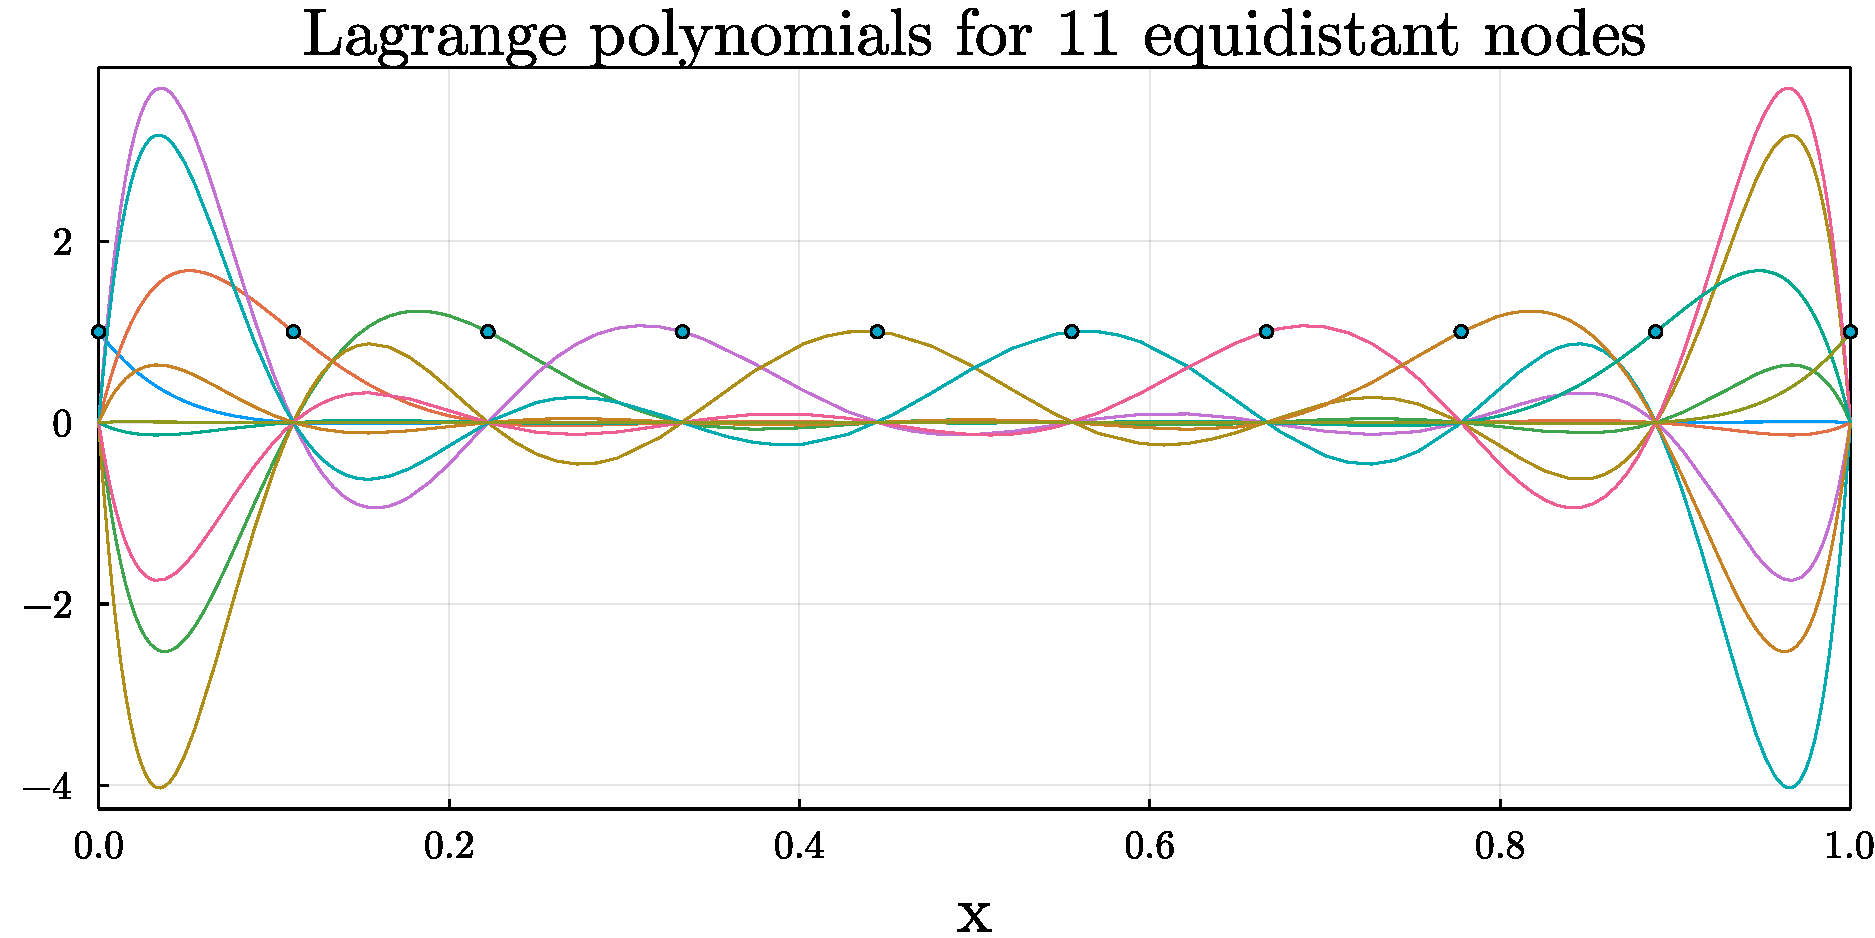
\includegraphics[width=0.8\linewidth]{figures/lagrange_10.pdf}
    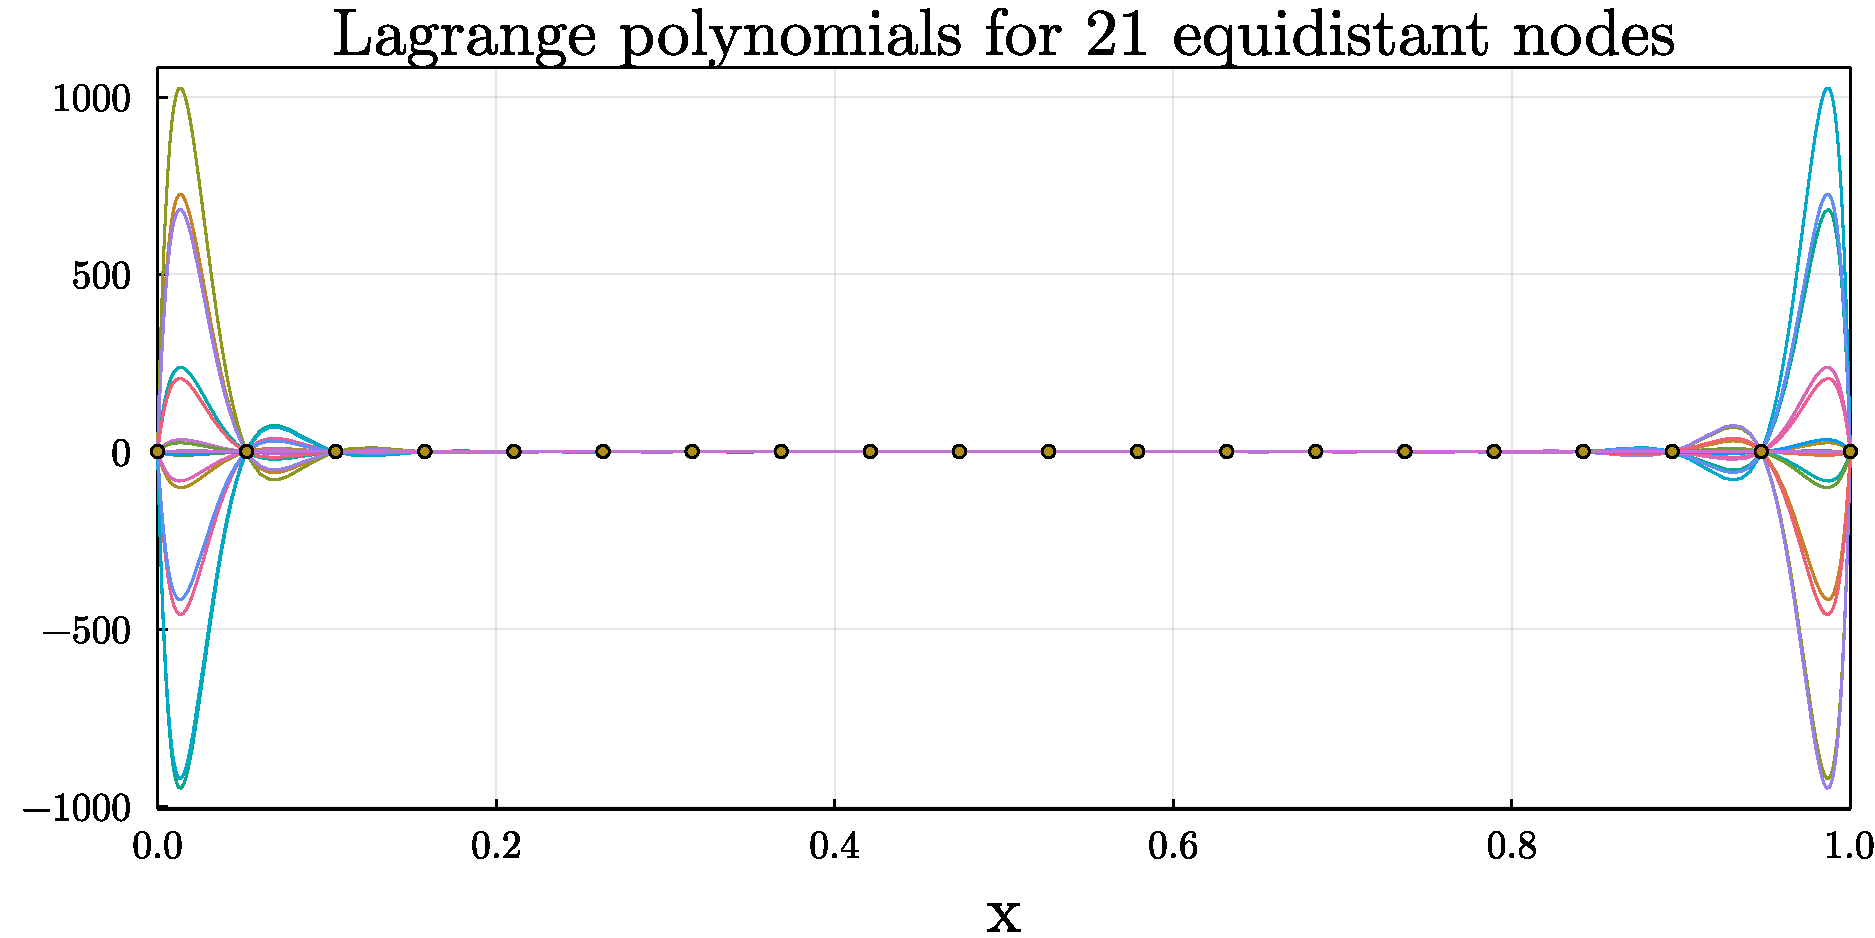
\includegraphics[width=0.8\linewidth]{figures/lagrange_20.pdf}
    \caption{Lagrange polynomials associated with equidistant nodes over the $(0, 1)$ interval.}%
    \label{fig:lagrange}
\end{figure}

\subsection{Gregory--Newton interpolation}
By Taylor's formula,
any polynomial~$p$ of degree $n$ may be expressed as
\begin{equation}
    \label{eq:taylor}
    p(x) = p(0) + p'(0) x + \frac{p''(0)}{2} x^2 + \dotsc + \frac{p^{(n)}(0)}{n!} x^n.
\end{equation}
The constant coefficient can be obtained by evaluating the polynomial at 0,
the linear coefficient can be identified by evaluating the first derivative at 0,
and so on.
Assume now that we are given the values taken by~$p$ when evaluated at the integer numbers $\{0, \dotsc, n\}$.
We ask the following question:
can we find a formula similar in spirit to~\eqref{eq:taylor},
but including only evaluations of $p$ and not of its derivatives?
To answer this question, we introduce the difference operator $\Delta$ which acts on functions as follows:
\[
    \Delta f(x) = f(x+1) - f(x).
    % (p_0, p_1, \dotsc) \mapsto (p_1 - p_0, p_2 - p_1, \dotsc).
\]
The operator~$\Delta$ is a linear operator on the space of continuous functions.
It maps constant functions to 0,
and the linear function~$x$ to the constant function~$1$,
suggesting a resemblance with the differentiation operator.
In order to further understand this connection,
let us define the \emph{falling power} of a real number $x$ as
\[
    x^{\underline{k}} = x (x-1) (x-2) \dots (x-k+1).
\]
We then have that
\begin{align*}
    \Delta x^{\underline{k}}
    &= (x+1) x (x-1) \dots (x-k+2) - x (x-1) (x-2) \dots (x-k+1) \\
    &= \bigl((x+1) - (x-k+1)\bigr) \bigl(x (x-1) \dots (x-k+2)\bigr) = k x^{\underline{k-1}}
\end{align*}
In other words,
the action of the difference operator on falling powers mirrors that of the differentiation operator on monomials.
The falling powers form a basis of the space of polynomials,
and so any polynomial in~$\poly(n)$, i.e.\ of degree less than or equal to $n$, can be expressed as
\begin{equation}
    \label{eq:gregory_newton}
    p(x) = \alpha_0 + \alpha_1 x^{\underline{1}} + \alpha_2 x^{\underline{2}} + \dotsb + \alpha_n x^{\underline{n}}.
\end{equation}
It is immediate to show that $\alpha_i = \Delta^i p(0)$,
where $\Delta^i p$ denotes the function obtained after~$i$ applications of the operator~$\Delta$.
Therefore, any polynomial of degree less than or equal to~$n$ may be expressed as
\begin{equation}
    \label{eq:gregory_newton_actually}
    p(x) = p(0) + \Delta p(0) x^{\underline{1}} + \frac{\Delta^2}{2} x^{\underline{2}} + \dotsb + \frac{\Delta^n p(0)}{n!} x^{\underline{n}}.
\end{equation}
An expansion of the form~\eqref{eq:gregory_newton_actually} is called a \emph{Newton series},
which is the discrete analog of the continuous Taylor series.
From the definition of~$\Delta$,
it is clear that the coefficients in~\eqref{eq:gregory_newton_actually} depend only on~$p(0), \dotsc, p(n)$.
We conclude that, given points $n+1$ points $(i, u_i)$ for $i \in \{0, \dotsc, n\}$,
the unique interpolating polynomial given by~\eqref{eq:gregory_newton_actually},
after replacing $p(i)$ by $u_i$.

\begin{example}
    \label{example:gregory_newton}
    Let us use~\eqref{eq:gregory_newton} in order to calculate the value of
    \[
        S(n) := \sum_{i=0}^{n} i^2.
    \]
    Since $\Delta S(n) = (n+1)^2$,
    which is a second degree polynomial in $n$,
    we deduce that $S(n)$ is a polynomial of degree 3.
    % Notice the slight abuse of notation here:
    % since $S(n)$ is well-defined only for $n \in \nat$,
    % $\Delta S(n)$ is also well-defined
    Let us now determine its coefficients.
    \begin{center}
    \begin{tabular}{|c|c|c|c|c|}
        \hline
        $n$    & $0$ & $1$ & $2$ & $3$ \\ \hline
        $\Delta^0 S(n)$ & $\mathbf{0}$ & $1$ & $5$ & $14$ \\ \hline
        $\Delta^1 S(n)$ & $\mathbf{1}$ & $4$ & $9$ &  \\ \hline
        $\Delta^2 S(n)$ & $\mathbf{3}$ & $5$ & & \\ \hline
        $\Delta^3 S(n)$ & $\mathbf{2}$ & & & \\ \hline
    \end{tabular}
    \end{center}
    We conclude that
    \[
        S(n) = \mathbf{1} n + \frac{\mathbf{3}}{2!} n(n-1) + \frac{\mathbf{2}}{3!} n(n-1)(n-2)
        = \frac{n (2n+1) (n+1)}{6}
    \]
\end{example}
Notice that when falling powers are employed as polynomial basis,
the matrix in~\eqref{eq:linear_system_interpolation} is lower triangular,
and so the algorithm described in~\cref{example:gregory_newton} could be replaced by the forward substitution method.
Whereas the coefficients of the Lagrange interpolant can be obtained immediately from the values of~$u$ at the nodes,
calculating the coefficients of the expansion in~\eqref{eq:gregory_newton} requires $\mathcal O(n^2)$ operations.
However, Gregory--Newton interpolation has several advantages over Lagrange interpolation:
\begin{itemize}
    \item
        If a point~$(n+1, p_{n+1})$ is added to the set of interpolation points,
        only one additional term, corresponding to the falling power~$x^{\underline{n+1}}$,
        needs to be calculated in~\eqref{eq:gregory_newton_actually}.
        All the other coefficients are unchanged.
        Therefore, the Gregory--Newton approach is well-suited for incremental interpolation.

    \item
        The Gregory--Newton interpolation method is more numerically stable than Lagrange interpolation,
        because the basis functions do not take very large values.

    \item
        A polynomial in the form of a Newton series can be evaluated efficiently using Horner's method,
        which is based on rewriting the polynomial as
        \[
            p(x) = \alpha_0 + x \biggl( \alpha_1 + (x-1)  \Bigl( \alpha_2 + (x-2)\bigl(\alpha_3 + (x-3) \dotsc \bigr) \Bigr)  \biggr).
        \]
        Evaluating this expression starting from the innermost bracket leads to an algorithm with a cost scaling linearly with the degree of the polynomial.
\end{itemize}

\subsubsection*{Non-equidistant nodes}%
So far,
we have described the Gregory--Newton method in the simple setting where interpolation nodes are just a sequence of successive natural numbers.
The method can be generalized to the setting of nodes $x_0 \neq \dotsc \neq x_n$ which are not necessarily equidistant.
In this case, we take as basis the following functions instead of the falling powers:
\begin{equation}
    \label{eq:basis_newton}
    \varphi_{i}(x) = (x - x_0) (x - x_1) \dotsc (x - x_{i-1}),
\end{equation}
with the convention that the empty product is 1.
By~\eqref{eq:linear_system_interpolation},
the coefficients of the interpolating polynomial in this basis solve the following linear system:
\begin{equation}
    \label{eq:matrix_newton}
    \begin{pmatrix}
        1 &         & \ldots &        & 0  \\
        1 & x_1-x_0 &        &        &    \\
        1 & x_2-x_0 & (x_2-x_0)(x_2-x_1) &        & \vdots   \\
        \vdots & \vdots  &        & \ddots &    \\
        1 & x_n-x_0 & \ldots & \ldots & \prod_{j=0}^{n-1}(x_n - x_j)
    \end{pmatrix}
    \begin{pmatrix}
        \alpha_0 \\
        \alpha_1 \\
        \alpha_2 \\
        \vdots \\
        \alpha_n
    \end{pmatrix}
    =
    \begin{pmatrix}
        u_0 \\
        u_1 \\
        u_2 \\
        \vdots \\
        u_n
    \end{pmatrix}.
\end{equation}
This system could be solved using, for example, forward substitution.
Clearly $\alpha_0 = u_0$,
and then from the second equation we obtain
\[
    \alpha_1 = \frac{u_1 - u_0}{x_1 - x_0} =: [u_0, u_1],
\]
which may be viewed as an approximation of the slope of~$u$ at $x_0$.
The right-hand side of this equation is an example of a \emph{divided difference}.
In general, divided differences are defined recursively as follows:
\[
    [u_{0}, u_{2}, \dotsc, u_{d}] := \frac{[u_{1}, \dotsc, u_{d}] - [u_{0}, \dotsc, u_{d-1}]}{x_{d}-x_{0}}, \qquad [u_i] = u_i.
\]
It is possible to find an expression for the coefficients of the interpolating polynomials in terms of these divided differences.
\begin{proposition}
    Assume that $(x_0, u_0), \dotsc, (x_n, u_n)$ are $n+1$ points in the plane with distinct abcissae.
    Then the interpolating polynomial of degree $n$ may be expressed as
    \[
        p(x) = \sum_{i=0}^{n} [u_0, \dotsc, u_n] \varphi_i(x),
    \]
    where $\varphi_i(x)$, for $i = 0, \dotsc, n$, are the basis functions defined in~\eqref{eq:basis_newton}.
\end{proposition}
\begin{proof}
    The statement is true for $n = 0$.
    Reasoning by induction, we assume that it holds true for polynomials of degree up to $n-1$.
    Let $p_1(x)$ and $p_2(x)$ be the interpolating polynomials at the points
    $x_0, x_1, \dotsc, x_{n-2}, x_{n-1}$ and $x_0, x_1, \dotsc, x_{n-2}, x_{n}$, respectively.
    Then
    \begin{equation}
        \label{eq:interpolating_polynomial}
        p(x) = p_1(x) + \frac{x - x_{n-1}}{x_n - x_{n-1}} \bigl(p_2(x) - p_1(x)\bigr)
    \end{equation}
    is a polynomial of degree~$n$ that interpolates all the data points.
    By the induction hypothesis,
    it holds that
    \begin{align*}
        p_1(x) &= u_0 + [u_0, u_1] (x - x_0) + \dotsc + [u_0, u_1, \dotsc, u_{n-2}, \mathbf{u_{n-1}}] \prod_{i=0}^{n-2} (x - x_i), \\
        p_2(x) &= u_0 + [u_0, u_1] (x - x_0) + \dotsc + [u_0, u_1, \dotsc, u_{n-2}, \mathbf{u_{n}}] \prod_{i=0}^{n-2} (x - x_i).
    \end{align*}
    Here we used bold font to emphasize the difference between the two expressions.
    Substituting these expressions in~\eqref{eq:interpolating_polynomial},
    we obtain
    \begin{align*}
        p(x) =
        &u_0 + [u_0, u_1] (x - x_0) + \dotsc + [u_0, \dotsc, u_{n-2}] \prod_{i=0}^{n-2} (x - x_i)  \\
        & + \frac{[u_0, u_1, \dotsc, u_{n-2}, u_{n-1}] - [u_0, u_1, \dotsc, u_{n-2}, u_{n}]}{x_n - x_{n-1}} \prod_{i=0}^{n-1} (x - x_i).
    \end{align*}
    In \cref{exercise:divided_differences},
    we show that divided differences are invariant under permutations of the data points,
    and so we have that
    \[
        \frac{[u_0, u_1, \dotsc, u_{n-2}, u_{n-1}] - [u_0, u_1, \dotsc, u_{n-2}, u_{n}]}{x_n - x_{n-1}} = [u_0, \dotsc, u_n],
    \]
    which enables to conclude.
\end{proof}
\begin{example}
    Assume that we are looking for the third degree polynomial going through the points
    \[
        (-1, 10), \qquad (0, 4), \qquad (2, -2), \qquad (4, -40).
    \]
    We have to calculate $\alpha_i = [u_0, \dotsc, u_i]$ for $i \in \{0, 1, 2, 3\}$.
    It is convenient to use a table in order to calculate the divided differences:
    \begin{center}
    \begin{tabular}{|c|c|c|c|c|}
        \hline
        $i$ & $0$ & $1$ & $2$ & $3$ \\ \hline
        $[u_i]$ & $\mathbf{10}$ & $4$ & $-2$ & $-40$ \\ \hline
        $x_{i+1} - x_{i}$ & $1$ & $2$ & $2$ &  \\ \hline
        $[u_i, u_{i+1}]$ & $\mathbf{-6}$ & $-3$ & $-19$ &  \\ \hline
        $x_{i+2} - x_{i}$ & $3$ & $4$ &  &  \\ \hline
        $[u_i, u_{i+1}, u_{i+2}]$ & $\mathbf{1}$ & $-4$ & & \\ \hline
        $x_{i+3} - x_{i}$ & $5$  & &  &  \\ \hline
        $[u_i, u_{i+1}, u_{i+2}, u_{i+3}]$ & $\mathbf{-1}$ & & & \\ \hline
    \end{tabular}
    \end{center}
    We deduce that the expression of the interpolating polynomial is
    \[
        p(x)
        = \mathbf{10} + (\mathbf{-6})(x+1) + \mathbf{1} (x+1)x + (\mathbf{-1}) (x+1)x(x-2)
        = - x^3 + 2 x^2 + -3x + 4.
    \]
\end{example}

\subsection{Interpolation error}
Assume that~$u(x)$ is a continuous function and denote by $\widehat u(x)$ its interpolation through the points~$(x_i, u_i)$,
for $i = 0, \dotsc, n$.
In this section, we study the behavior of the error in the limit as $n \to \infty$.

\begin{theorem}
    [Interpolation error]
    \label{theorem:interpolation_error}
    Assume that~$u\colon [a, b] \to \real$ is a function in $C^{n+1}([a, b])$ and let~$x_0, \dotsc, x_n$ denote $n+1$ distinct interpolation nodes.
    Then for all $x \in [a, b]$,
    there exists~$\xi = \xi(x)$ in the interval $[a, b]$ such that
    \[
        e_n(x) := u(x) - \widehat u(x) = \frac{u^{(n+1)}(\xi)}{(n+1)!} (x-x_0) \dotsc (x - x_n).
    \]
\end{theorem}
\begin{proof}
    The statement is obvious if $x \in \{x_0, \dotsc, x_n\}$,
    so we assume from now on that $x$ does not coincide with an interpolation node.
    Let us use the compact notation $\omega_n = \prod_{i=0}^n (x - x_i)$ and introduce the function
    \begin{equation}
        \label{eq:interpolation_error}
        g(t) = e_n(t) \omega_n(x) - e_n(x) \omega_n(t).
    \end{equation}
    The function $g$ is smooth and takes the value~0 when evaluated at~$x_0, \dotsc, x_n, x$.
    Since $g$ has $n+2$ roots in the interval $[a, b]$,
    Rolle's theorem implies that $g'$ has $n+1$ distinct roots in~$(a, b)$.
    Another application of Rolle's theorem yields that $g''$ has $n$ distinct roots in~$(a, b)$.
    Iterating this reasoning, we deduce that $g^{(n+1)}$ has one root~$t_*$ in $(a, b)$.
    From~\eqref{eq:interpolation_error},
    we calculate that
    \begin{equation}
        \label{eq:interpolation_error_proof}
        g^{(n+1)}(t) = e_n^{(n+1)}(t) \omega_n(x) - e_n(x) \omega_n^{(n+1)}(t)
        = u^{(n+1)}(t) \omega_n(x) - e_n(x) (n+1)!.
    \end{equation}
    Here we employed the fact that $\widehat u^{(n+1)}(t) = 0$,
    because $\widehat u$ is a polynomial of degree at most $n$.
    Evaluating~\eqref{eq:interpolation_error_proof} at~$t_*$ and rearranging,
    we obtain that
    \[
        e_n(x) = \frac{u^{(n+1)}(t_*)}{(n+1)!} \omega_n(x),
    \]
    which completes the proof.
\end{proof}
As a corollary to~\cref{theorem:interpolation_error},
we deduce the following error bound.
\begin{corollary}
    [Upper bound on the interpolation error]
    \label{corollary:interpolation_error}
    Assume that $u$ is smooth in $[a, b]$ and that
    \[
        \sup_{x \in [a, b]} \abs{u^{(n+1)}(x)} \leq C_{n+1}.
    \]
    Then
    \begin{equation}
        \label{eq:upper_bound_interp_error}
        \forall x \in [a, b], \qquad
        \abs{e_n(x)} \leq \frac{C_{n+1}}{4(n+1)} h^{n+1}
    \end{equation}
    where $h$ is the maximum spacing between two successive interpolation nodes.
\end{corollary}
\begin{proof}
By~\cref{theorem:interpolation_error},
we have
\begin{equation}
    \label{eq:bound_error_from_theorem}
    \forall x \in [a, b], \qquad
    \abs{e_n(x)} \leq \frac{C_{n+1}}{(n+1)!} \abs[Big]{(x-x_0) \dotsc (x-x_n)}.
\end{equation}
The product on the right-hand side is bounded from above by
\begin{equation}
    \label{eq:interpolation_bound_product}
    \frac{h^2}{4} \times 2h \times 3h \times 4h \times \dotsb \times nh = \frac{n! h^{n+1}}{4}.
\end{equation}
The first factor comes from the fact that, if $x \in [x_i, x_{i+1}]$,
then
\[
    \abs{(x - x_i)(x - x_{i+1})} \leq \frac{(x_{i+1} - x_i)^2}{4},
\]
because the left-hand side is maximized when $x$ is the midpoint of the interval~$[x_i, x_{i+1}]$.
Substituting~\eqref{eq:interpolation_bound_product} into~\eqref{eq:bound_error_from_theorem},
we deduce the statement.
\end{proof}
Let us now introduce the supremum norm of the error over the interval $[a, b]$:
\[
    E_n = \sup_{x \in [a, b]} \abs{e_n(x)}.
\]
We ask the following natural question:
does $E_n$ tend to zero as the maximum spacing between successive nodes tends to 0?
By~\cref{corollary:interpolation_error},
the answer to this question is positive when $C_{n}$ does not grow too quickly as $n \to \infty$.
For example, as illustrated in \cref{fig:interpolation_sine},
the interpolation error for the function $u(x) = \sin(x)$,
when using equidistant interpolation nodes,
decreases very quickly as $n \to \infty$.
\begin{figure}[ht!]
    \centering
    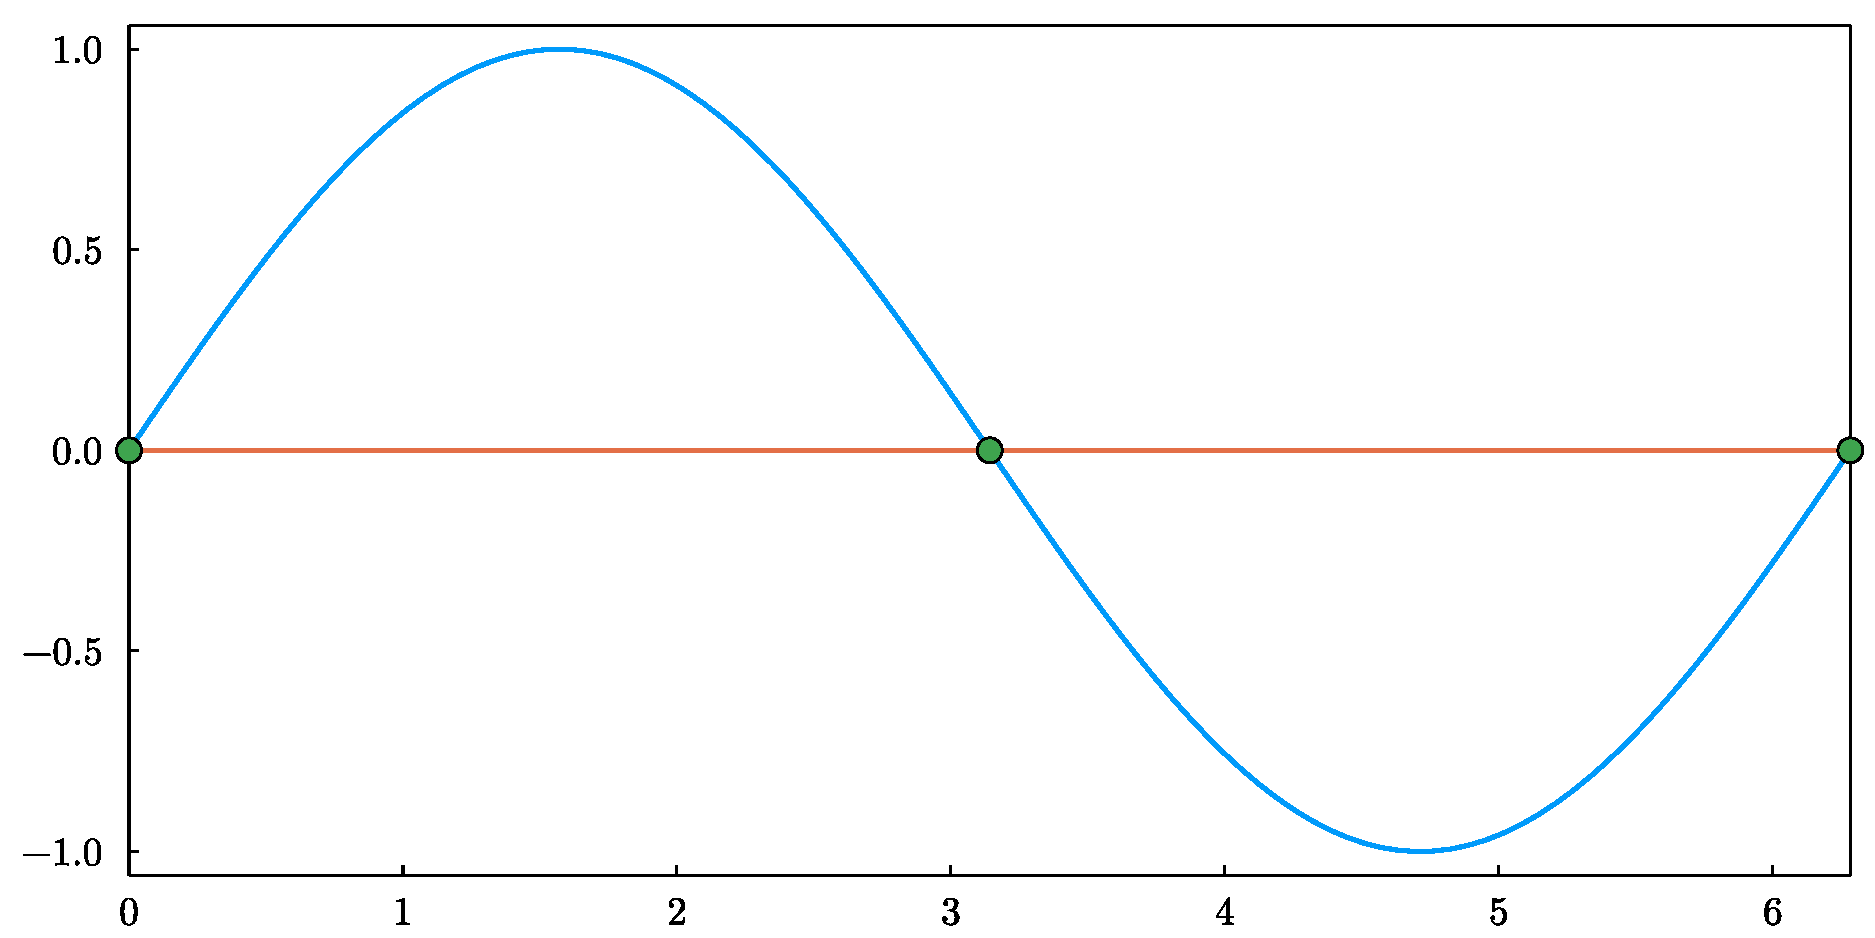
\includegraphics[width=0.49\linewidth]{figures/interpolation_sine_3.pdf}
    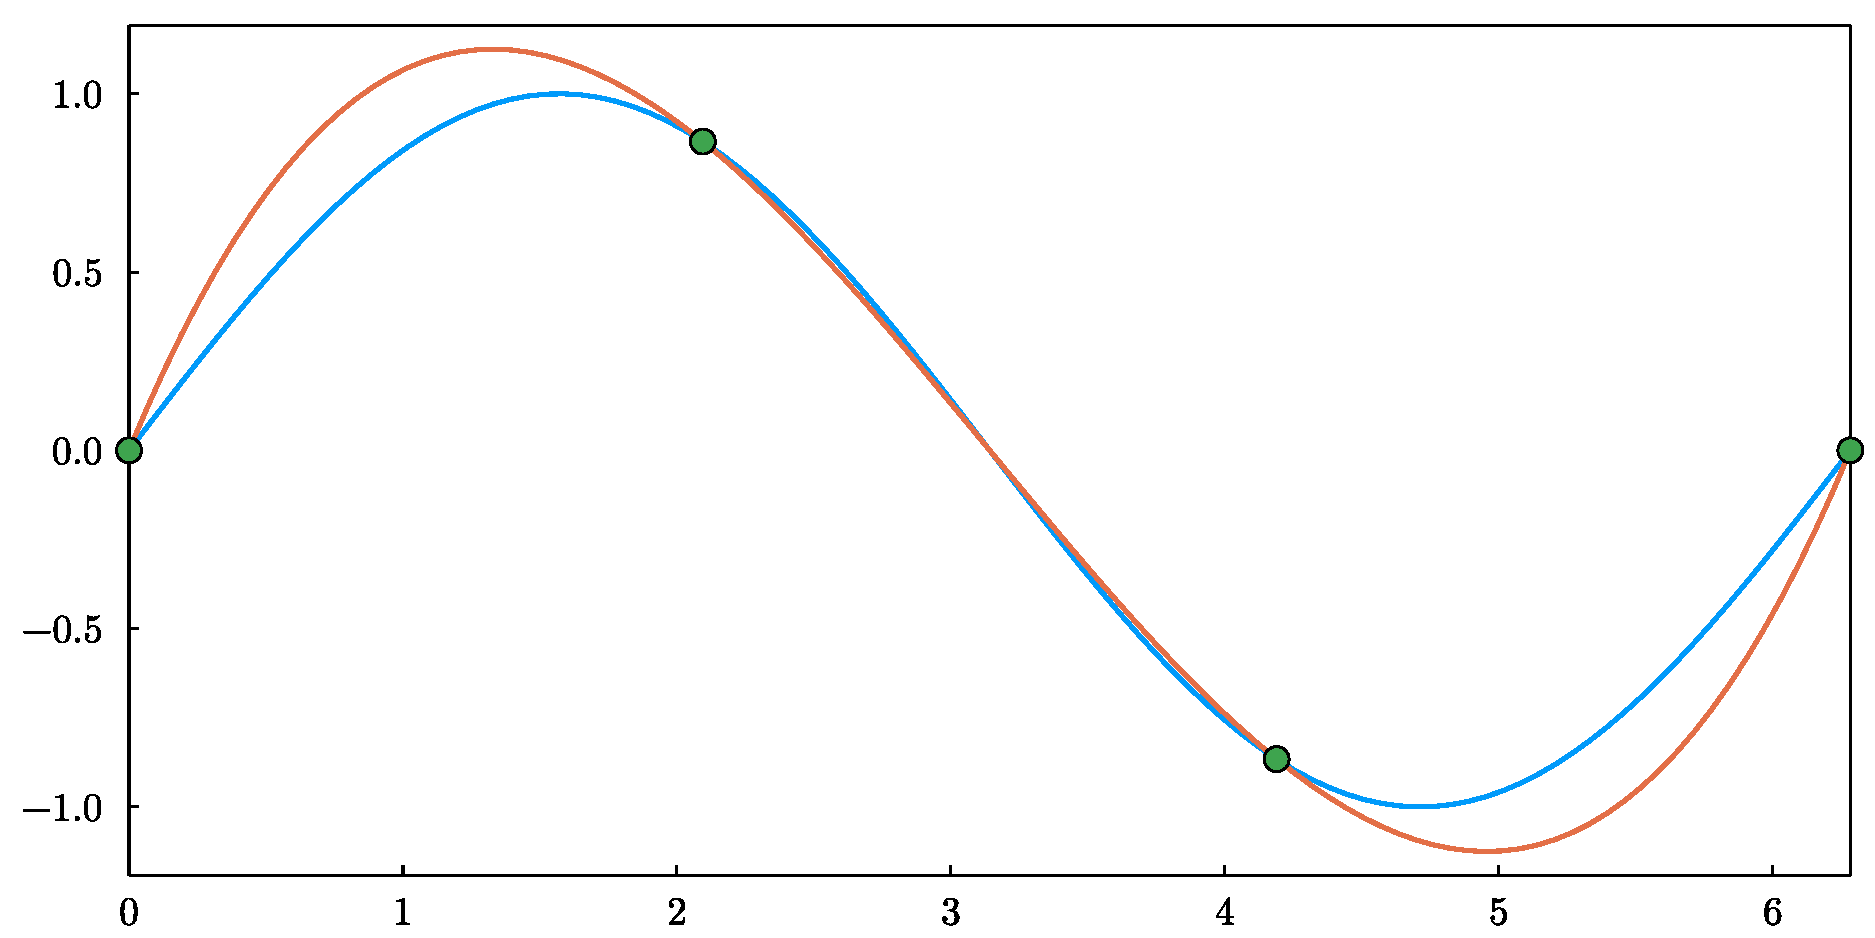
\includegraphics[width=0.49\linewidth]{figures/interpolation_sine_4.pdf}
    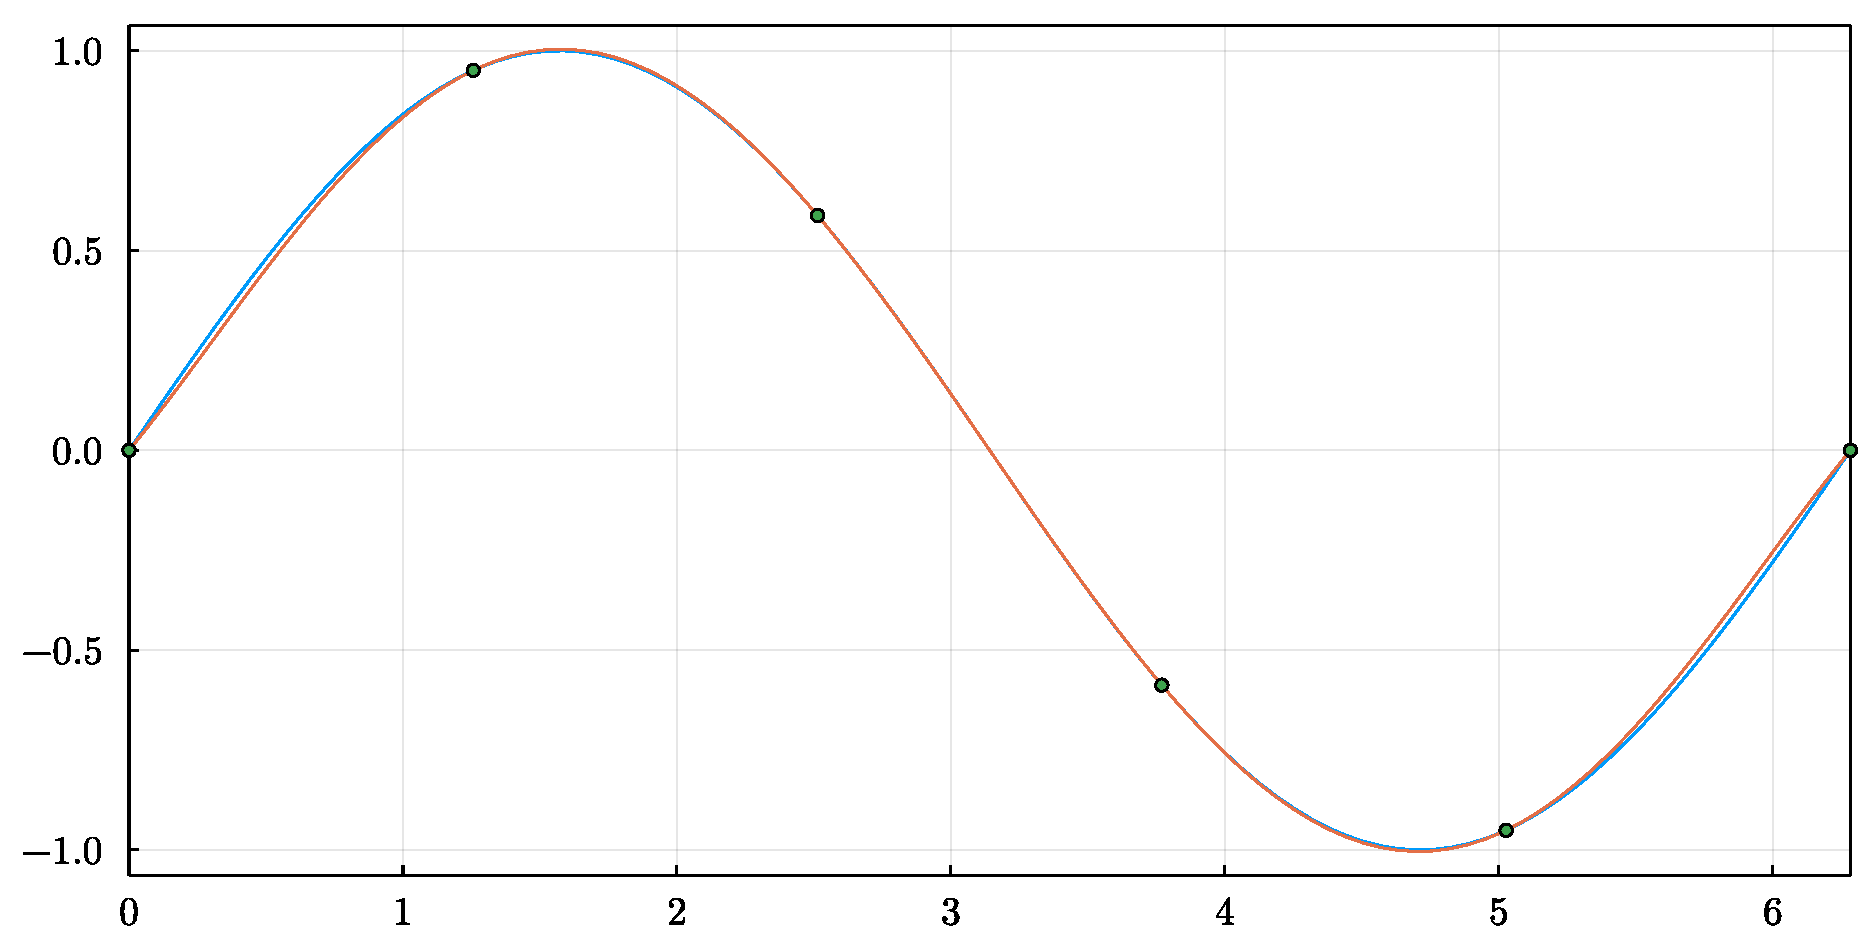
\includegraphics[width=0.49\linewidth]{figures/interpolation_sine_6.pdf}
    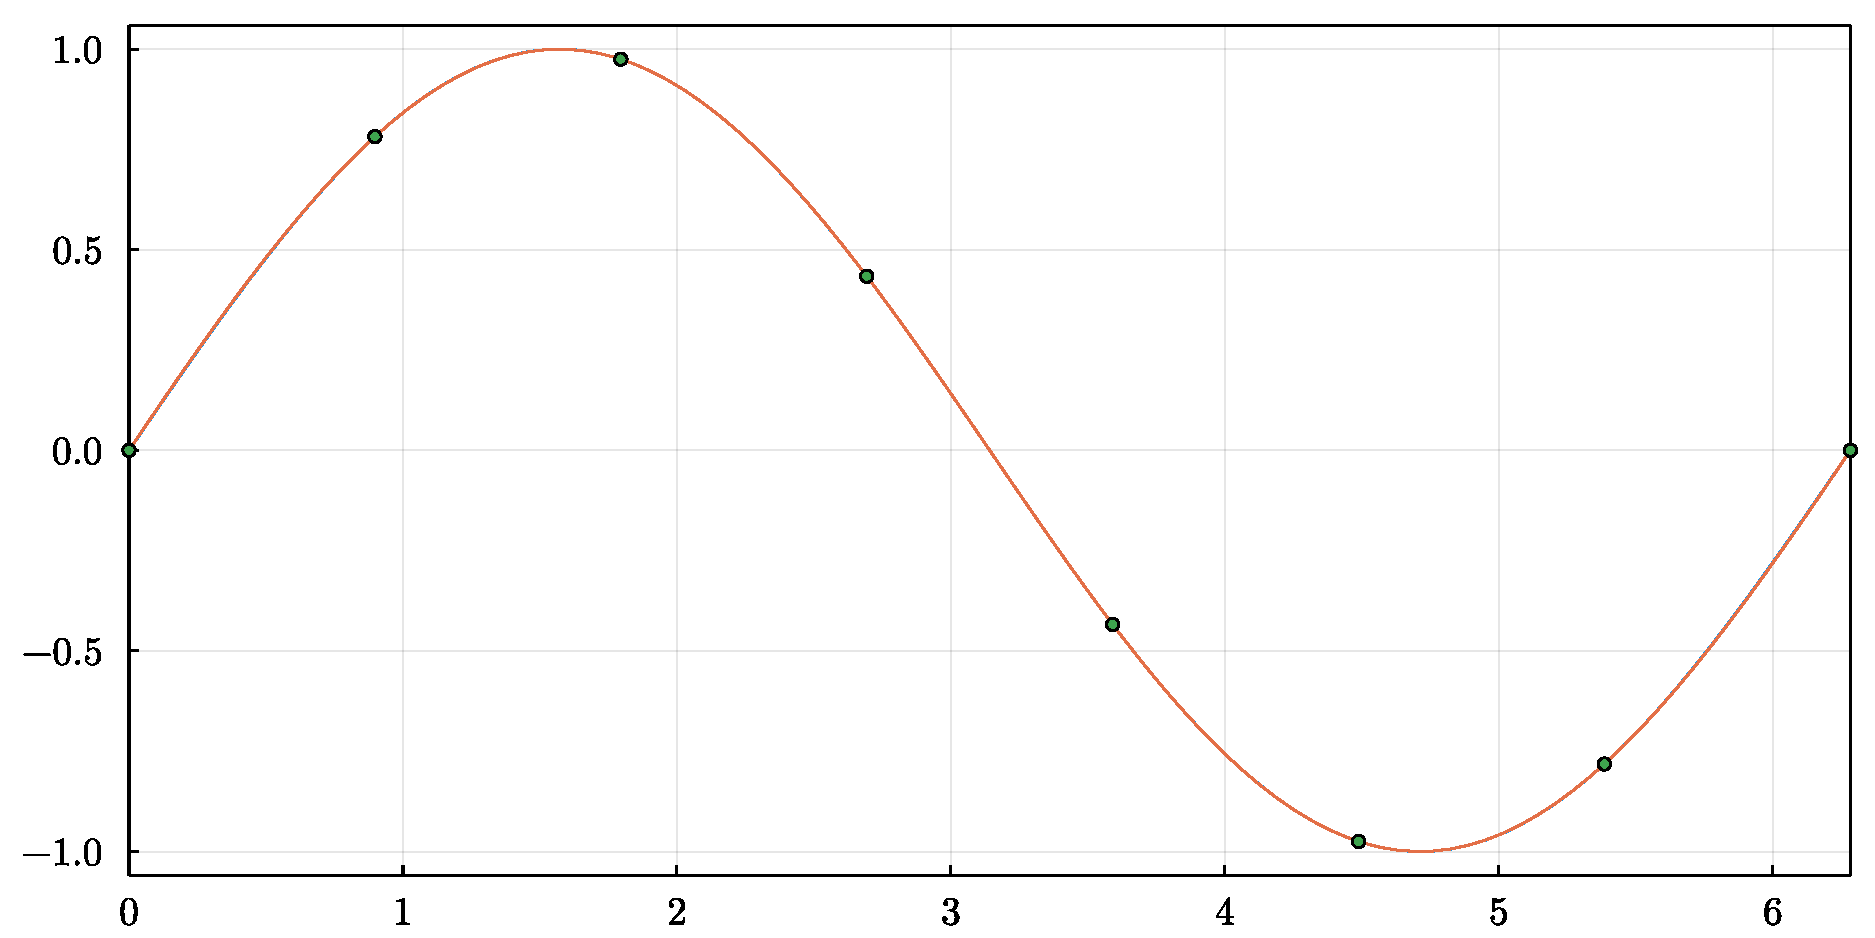
\includegraphics[width=0.49\linewidth]{figures/interpolation_sine_8.pdf}
    \caption{Interpolation (in orange) of the function $u(x) = \sin(x)$ (in blue) using 3, 4, 6, and 8 equidistant nodes.}%
    \label{fig:interpolation_sine}
\end{figure}

In some cases, however,
the constant $C_n$ grows quickly with $n$,
to the extent that $E_n$ may increase with $n$;
in this case, the maximum interpolation error grows as we add nodes!
The classic example,
in order to illustrate this potential issue,
is that of the Runge function:
\begin{equation}
    \label{eq:runge_function}
    u(x) = \frac{1}{1 + 25 x^2}.
\end{equation}
It is possible to show that,
for this function,
the upper bound in~\cref{corollary:interpolation_error} tends to $\infty$ in the limit as the number of interpolation nodes increases.
We emphasize that this does not prove that $E_n \to \infty$ in the limit as $n \to \infty$,
because~\eqref{eq:upper_bound_interp_error} provides only an \emph{upper bound} on the error.
In fact, the interpolation error for the Runge function can either grow or decrease,
depending on the choice of interpolation nodes.
With equidistant nodes, it turns out that $E_n \to \infty$,
as illustrated in~\cref{fig:interpolation_runge_function}.
\begin{figure}[ht!]
    \centering
    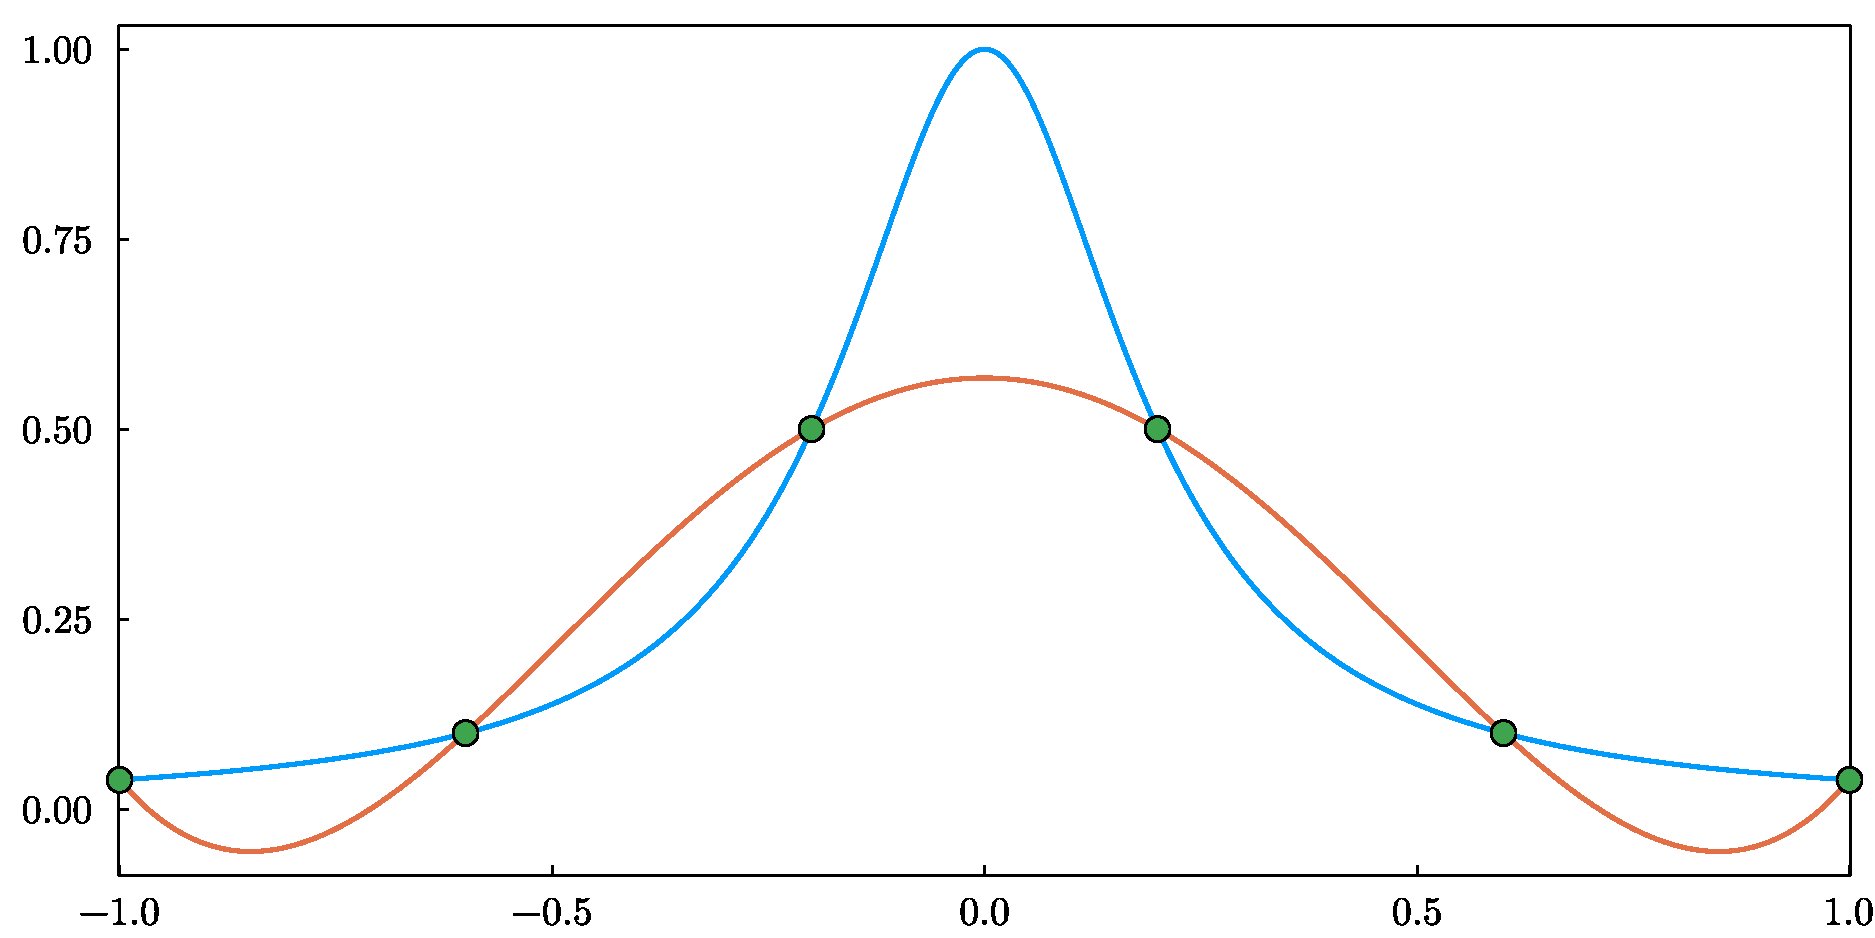
\includegraphics[width=0.49\linewidth]{figures/interpolation_runge_6.pdf}
    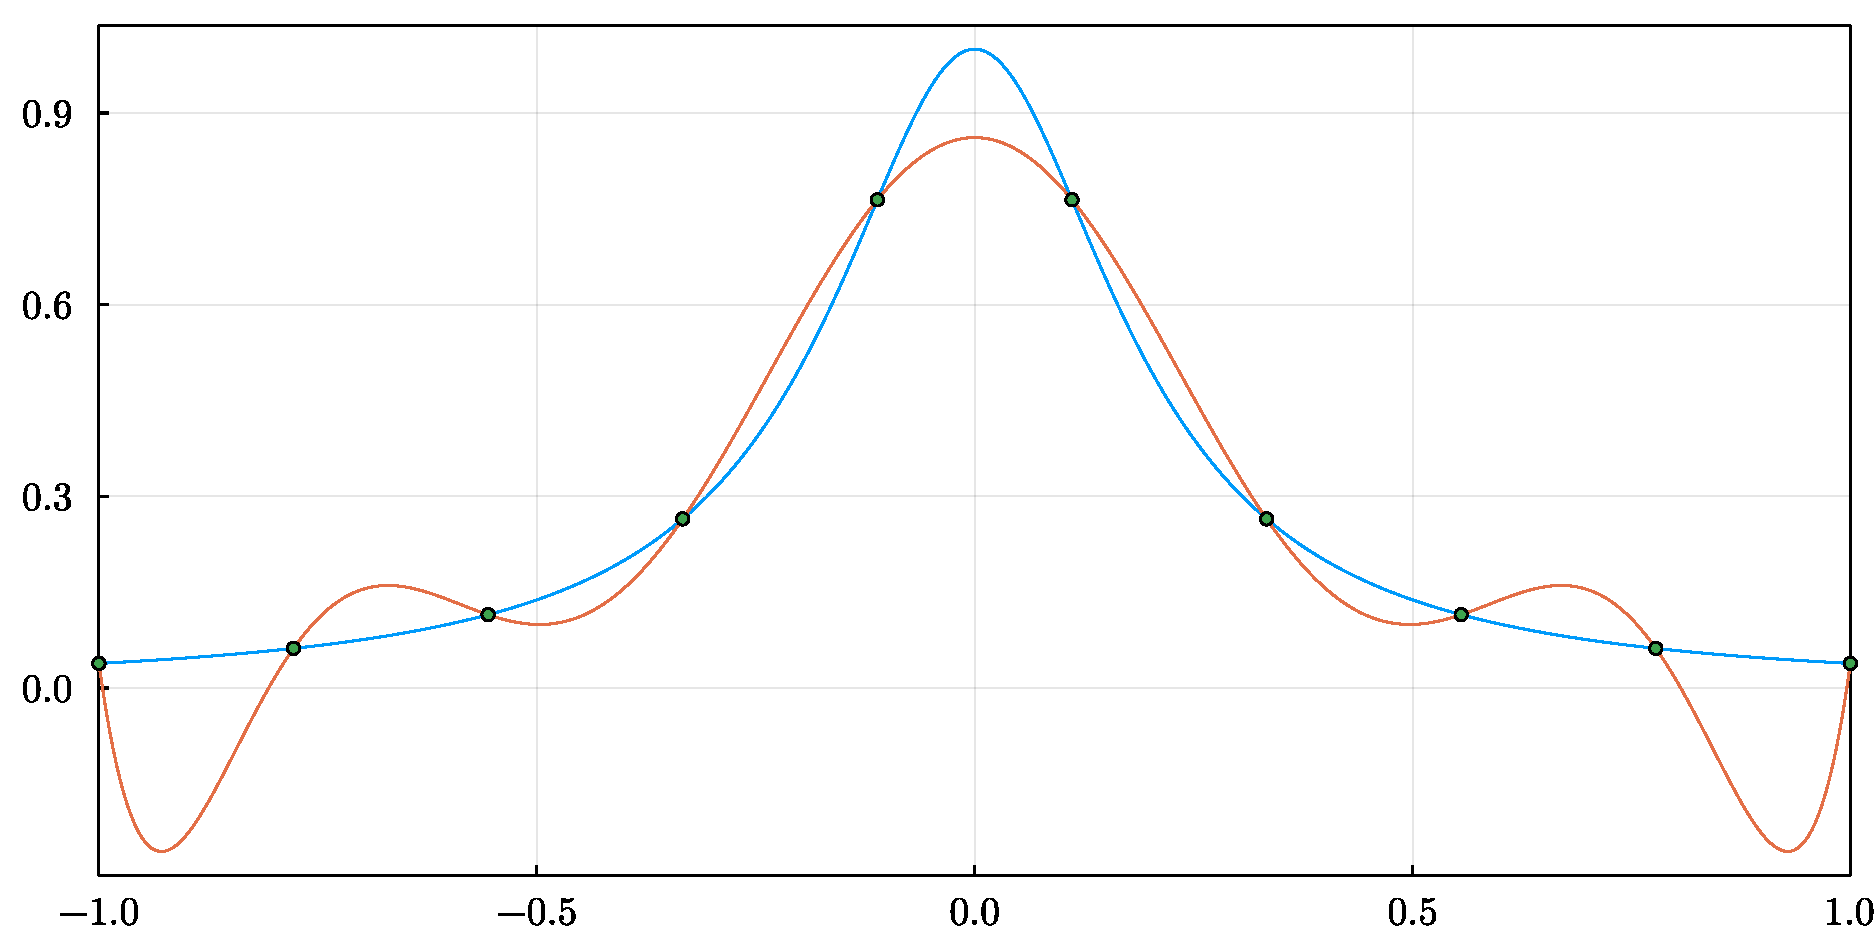
\includegraphics[width=0.49\linewidth]{figures/interpolation_runge_10.pdf}
    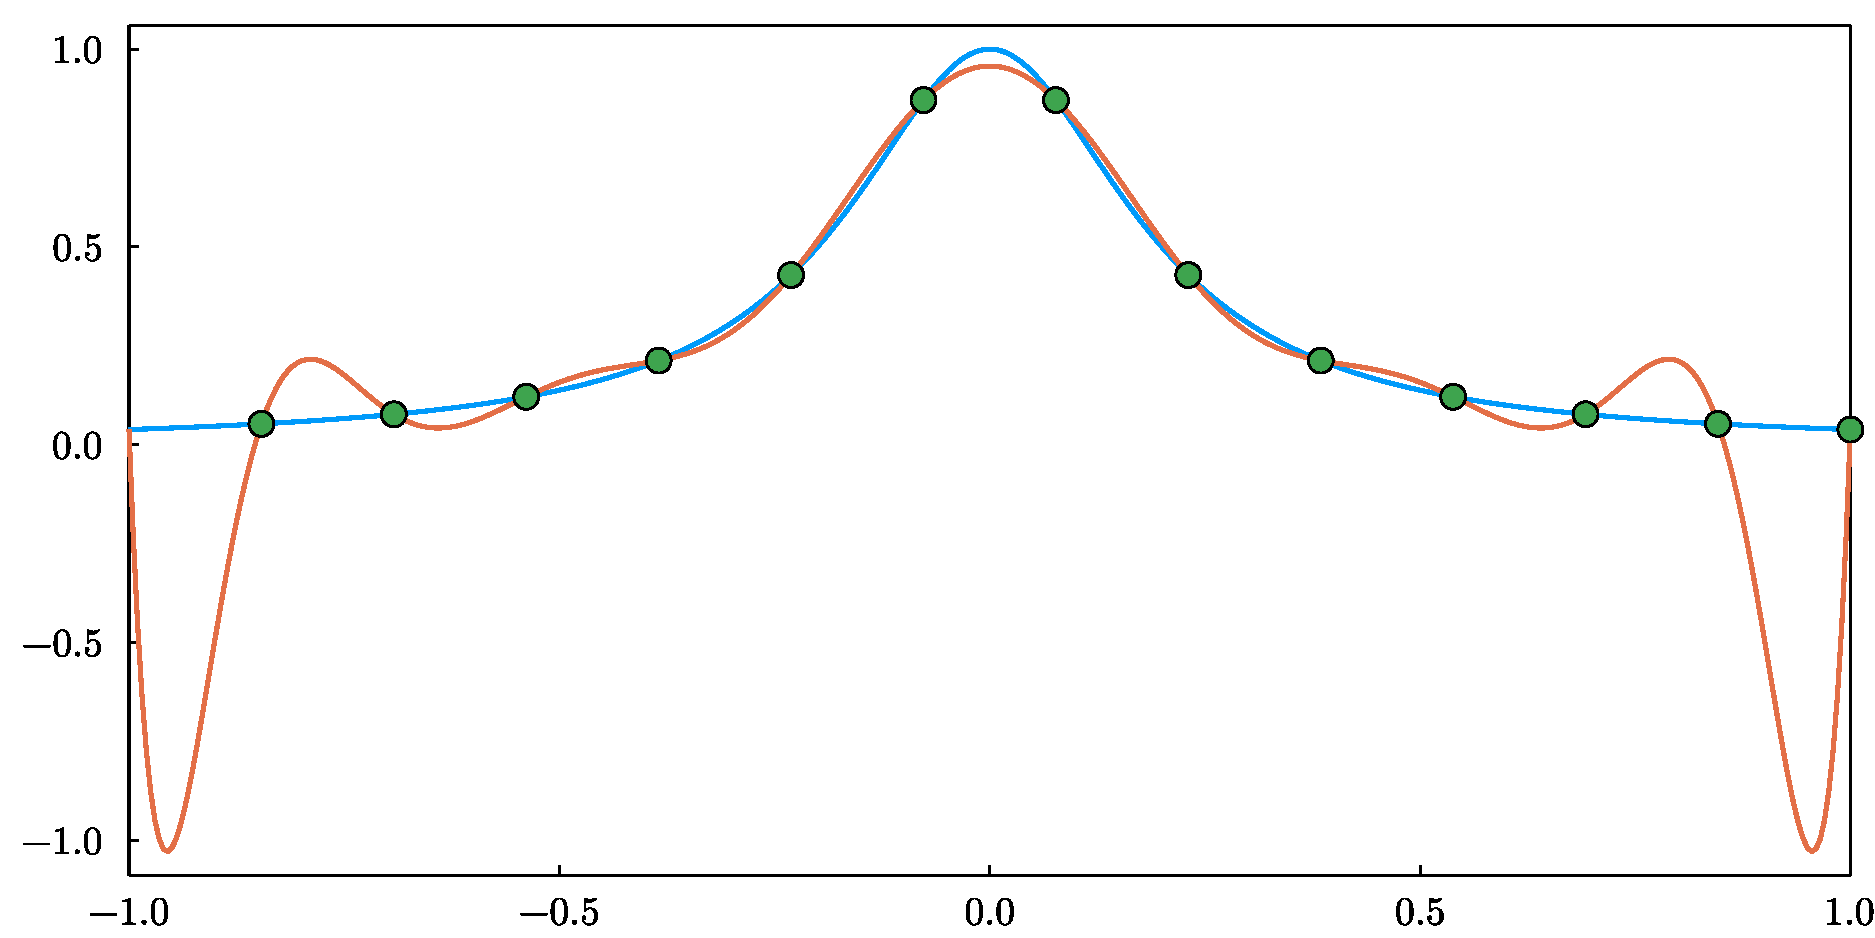
\includegraphics[width=0.49\linewidth]{figures/interpolation_runge_14.pdf}
    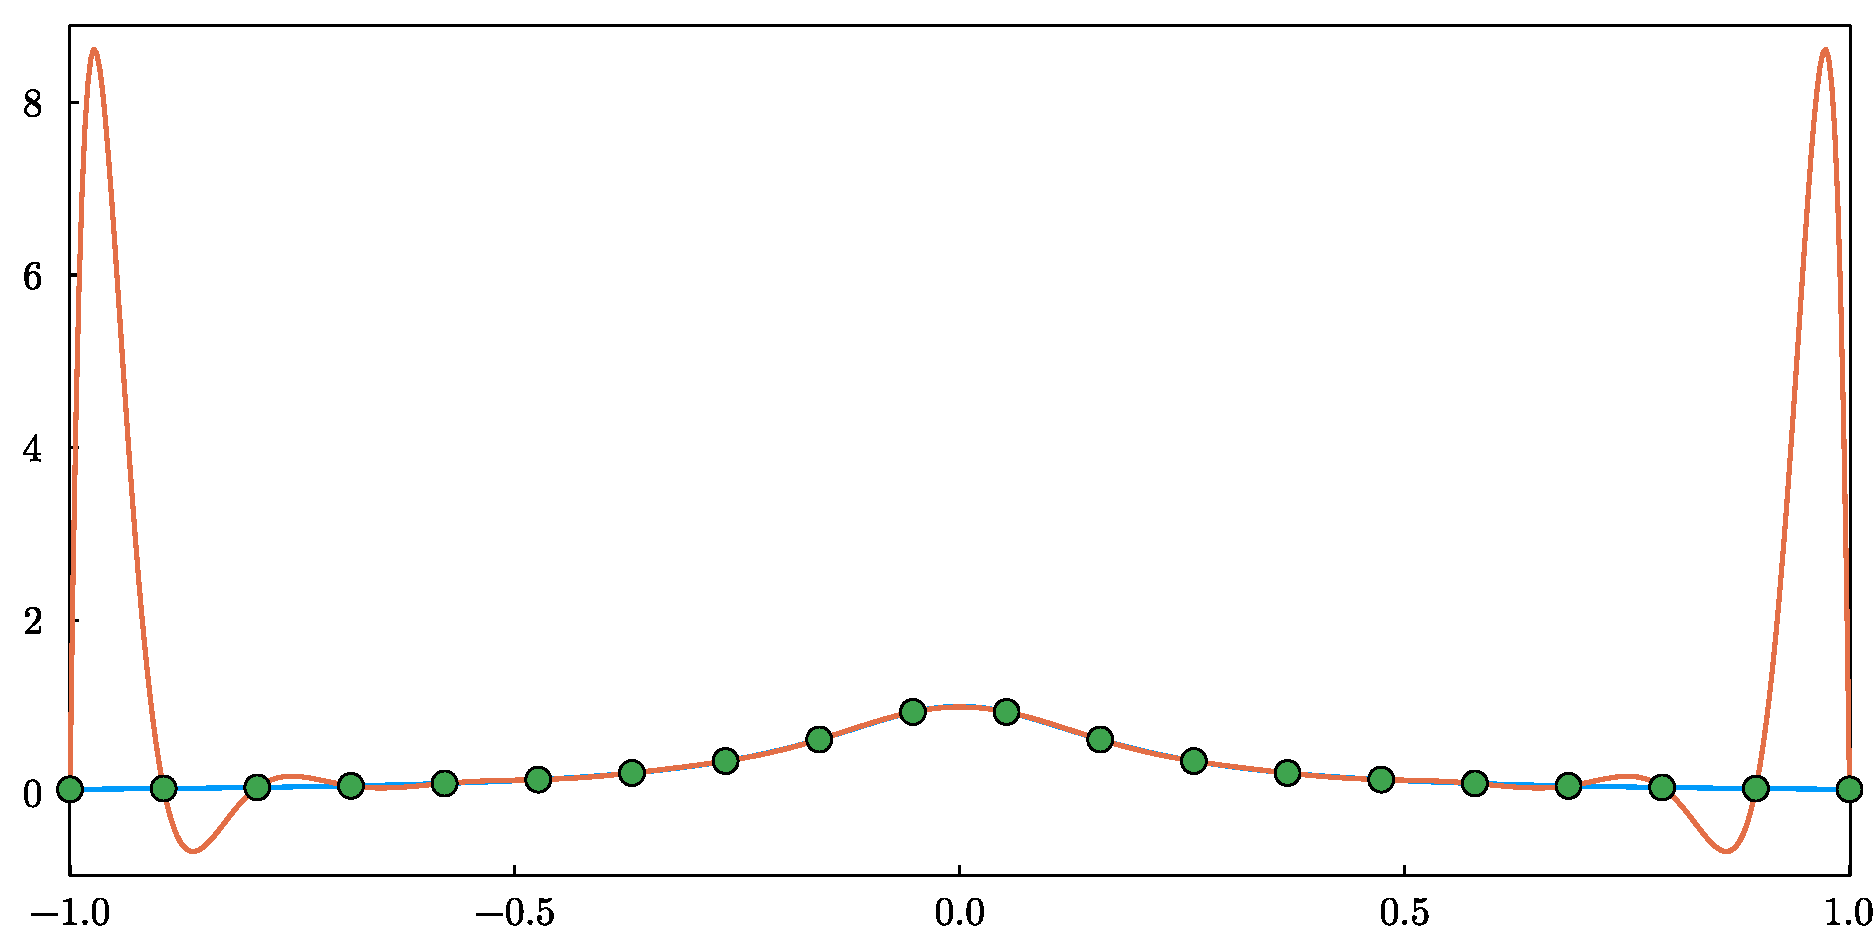
\includegraphics[width=0.49\linewidth]{figures/interpolation_runge_20.pdf}
    \caption{Interpolation (in orange) of the Runge function~\eqref{eq:runge_function} (in blue) using 6, 10, 14, and 20 equidistant nodes.}%
    \label{fig:interpolation_runge_function}
\end{figure}

\subsection{Interpolation at Chebyshev nodes}
Sometimes,
interpolation is employed as a technique for approximating functions.
The spectral collocation method, for example,
is a technique for solving partial differential equations
where a discrete solution is first calculated,
and then a continuous solution is constructed using polynomial or Fourier interpolation.
When the interpolation nodes are not given a priori as data,
it is natural to wonder whether these can be picked in such a manner that the interpolation error,
measured in a function norm, is minimized.
For example, given a continuous function~$u(x)$ and a number of nodes~$n$,
is it possible to chose nodes $x_0, \dotsc, x_n$ such that
\[
    E := \sup_{x \in [a, b]} \abs{u(x) - \widehat u(x)}
\]
is minimized?
Here $\widehat u$ is the polynomial interpolating~$u$ at the nodes.
Achieving this goal in general is a difficult task,
essentially because $\xi = \xi(x)$ is unknown in the expression of the interpolation error from~\cref{theorem:interpolation_error}:
\[
    e_n(x) = \frac{u^{(n+1)}(\xi)}{n+1!} (x-x_0) \dotsc (x - x_n).
\]
In view of this difficulty,
we will focus on the simpler problem of finding interpolation nodes
such that the product $(x-x_0) \dotsc (x - x_n)$ is minimized in the supremum norm.
This problem amounts to finding the optimal interpolation nodes,
in the sense that~$E$ is minimized,
in the particular case where $u$ is a polynomial of degree $n+1$,
because in this case $u^{n+1}(\xi)$ is a constant factor.
It turns out that this problem admits an explicit solution,
which we will deduce from the following theorem.
\begin{theorem}
    [Minimum $\infty$ norm]
    \label{theorem:minimum_infty_norm}
    Assume that $p$ is a monic polynomial of degree $n$:
    \[
        p(x) = \alpha_0 + \alpha_1 x + \dotsb + \alpha_{n-1} x^{n-1} + \mathbf{1} x^n.
    \]
    Then it holds that
    \begin{equation}
        \label{eq:chebychev_lower_bound}
        \sup_{x \in [-1, 1]} \abs{p(x)} \geq \frac{1}{2^{n-1}} =: E.
    \end{equation}
    In addition, the lower bound is achieved for~$p_*(x) = 2^{-(n-1)} T_n(x)$,
    where $T_n$ is the Chebyshev polynomial of degree~$n$:
    \begin{equation}
        \label{eq:chebyshev_polynomial}
        T_n(x) = \cos(n\arccos x) \qquad (-1 \leq x \leq 1).
    \end{equation}
\end{theorem}
\begin{proof}
    By~\cref{exercise:chebychev},
    the polynomial $x \mapsto 2^{-(n-1)} T_n(x)$ is indeed monic,
    and it is clear that it achieves the lower bound~\eqref{eq:chebychev_lower_bound}
    since $\abs{T_n(x)} \leq 1$.

    In order to prove~\eqref{eq:chebychev_lower_bound},
    we assume by contradiction that there is a different monic polynomial~$\widetilde p$ of degree~$n$ such that
    \begin{equation}
        \label{eq:chebyshev_minimum}
        \sup_{x \in [-1, 1]} \abs{\widetilde p(x)} < E.
    \end{equation}
    Let us introduce $x_i = \cos(i \pi/n)$, for $i = 0, \dotsc, n$,
    and observe that
    \[
        p(x_i) = 2^{-(n-1)} T_n(x_i) = (-1)^i E.
    \]
    The function $q(x) := p(x) - \widetilde p(x)$ is a polynomial of degree at most $n-1$ which,
    by the assumption~\eqref{eq:chebyshev_minimum},
    is strictly positive at $x_0, x_2, x_4, \dotsc$ and strictly negative at $x_1, x_3, x_5, \dotsc$.
    Therefore, the polynomial $q(x)$ changes sign at least $n$ times and so,
    by the intermediate value theorem, it has at least $n$ roots.
    But this is impossible, because $q(x) \neq 0$ and $q(x)$ is of degree at most $n-1$.
\end{proof}
\begin{remark}
    [Derivation of Chebyshev polynomials]
    \label{remark:cheb}
    The polynomial~$p_*$ achieving the lower bound in~\eqref{eq:chebychev_lower_bound}
    oscillates between the values $-E$ and $E$,
    which are respectively its minimum and maximum values over the interval~$[-1, 1]$.
    It attains the values $E$ or $-E$ at $n+1$ points $x_0, \dotsc, x_n$,
    with $x_0 = -1$ and $x_n = 1$.
    It turns out that these properties,
    which can be shown to hold a priori using Chebyshev's \emph{equioscillation theorem},
    are sufficient to derive an explicit expression for the polynomial~$p_*$,
    as we formally demonstrate hereafter.

    The points $x_2, \dotsc, x_{n-1}$
    are local extrema of~$p_*$,
    and so~$p_*'(x) = 0$ at these nodes.
    We therefore deduce that $p_*$ satisfies the differential equation
    \begin{equation}
        \label{eq:differential_equation_chebyshev}
        n^2\bigl(E^2 - p_*(x)^2\bigr) = p_*'(x)^2 (1 - x^2).
    \end{equation}
    Indeed, both sides are polynomials of degree $2n$ with single roots at -1 and 1,
    with double roots at $x_2, \dotsc, x_{n+1}$,
    and with the same coefficient of the leading power.
    In order to solve~\eqref{eq:differential_equation_chebyshev},
    we rearrange the equation and take the square root:
    \[
        \frac{\frac{p_*'(x)}{E}}{\sqrt{1 - \frac{p_*(x)^2}{E^2}}} = \pm \frac{n}{1 - x^2}
        \qquad \Leftrightarrow \qquad
        \frac{\d}{\d x} \arccos\left(\frac{p_*(x)}{E}\right) = \pm n \frac{\d}{\d x} \arccos(x).
    \]
    Integrating both sides and taking the cosine,
    we obtain
    \[
        p_*(x) = E \cos\bigl(C + n \arccos(x)\bigr).
    \]
    Requiring that $|p_*(-1)| = E$, we deduce $C = 0$.
\end{remark}

From~\cref{theorem:minimum_infty_norm},
we deduce the following corollary.
\begin{corollary}
    [Chebyshev nodes]
    \label{corollary:chebyshev_nodes}
    Assume that $x_0 < x_1 < \dotsc < x_n$ are in the interval $[a, b]$.
    The supremum norm of the product $\omega(x) := (x-x_0) \dotsb (x-x_n)$ over~$[a, b]$ is minimized when
    \begin{equation}
        x_i = a + (b-a) \frac{1 + \cos \left( \frac{(2i + 1) \pi}{2(n+1)} \right)}{2}
    \end{equation}
        % \label{eq:optimal_product}
        % (x-x_0) \dotsb (x-x_n) = \frac{(b-a)^n}{2^{2n-1}} T_n\left(\frac{a + b - 2x}{a - b}\right).
    % \end{equation}
    % In particular, if $a = -1$ and $b = 1$,
    % then the nodes $x_0, \dotsc, x_n$ must coincide with the roots of the Chebyshev polynomial of degree~$n$:
    % \[
        % x_i = \cos \left( (2i + 1) \frac{\pi}{2} \right).
    % \]
\end{corollary}
\begin{proof}
    We consider the affine change of variable
    \begin{align*}
        \zeta\colon &[-1, 1] \to [a, b]; \\
                    &y \mapsto \frac{a + b + y (b - a)}{2}.
    \end{align*}
    The function
    \begin{align*}
        p(y) &:= \frac{2^n}{(b-a)^n} \omega\bigl(\zeta(y)\bigr) = \frac{2^{n+1}}{(b-a)^{n+1}} \bigl(\zeta(y)-x_0\bigr) \dotsb \bigl(\zeta(y)-x_n\bigr) \\
             &= \bigl(y-y_0\bigr) \dotsb \bigl(y-y_n\bigr), \qquad y_i = \zeta^{-1}(x_i),
    \end{align*}
    is a monic polynomial of degree~$n+1$ such that
    \begin{equation}
        \label{eq:change_of_variable}
        \sup_{y \in [-1, 1]} \abs{p(y)} = \frac{2^{n+1}}{(b-a)^{n+1}} \sup_{x \in [a, b]} \abs{(x-x_0) \dotsc (x - x_n)}.
    \end{equation}
    By~\cref{theorem:minimum_infty_norm},
    the left-hand side is minimized when $p$ is equal to $2^{-n} T_{n+1}(y)$,
    i.e.\ when the roots of $p$ coincide with the roots of $T_{n+1}$.
    This occurs when
    \[
        y_i = \zeta^{-1}(x_i) = \cos \left( \frac{(2i + 1)\pi}{2 (n+1)} \right).
    \]
    Applying the inverse change of variable $x_i = \zeta(y_i)$,
    we deduce the result.
\end{proof}

\Cref{corollary:chebyshev_nodes} is useful for interpolation.
The nodes
\begin{equation}
    x_i = a + (b-a) \frac{1 + \cos \left( (2i + 1) \frac{\pi}{2 n} \right)}{2}, \qquad i = 0, \dotsc, n,
\end{equation}
are known as Chebyshev nodes and,
more often than not, employing these nodes for interpolation produces much better results than using equidistant rodes,
both in the case where~$u$ is a polynomial of degree $n+1$,
as we just proved,
but also for general~$u$.
As an example we plot in \cref{fig:cheb_runge} the interpolation of the Runge function using Chebyshev nodes.
In this case, the interpolating polynomial converges uniformly to the Runge function as we increase the number of interpolation nodes!
\begin{figure}[ht]
    \centering
    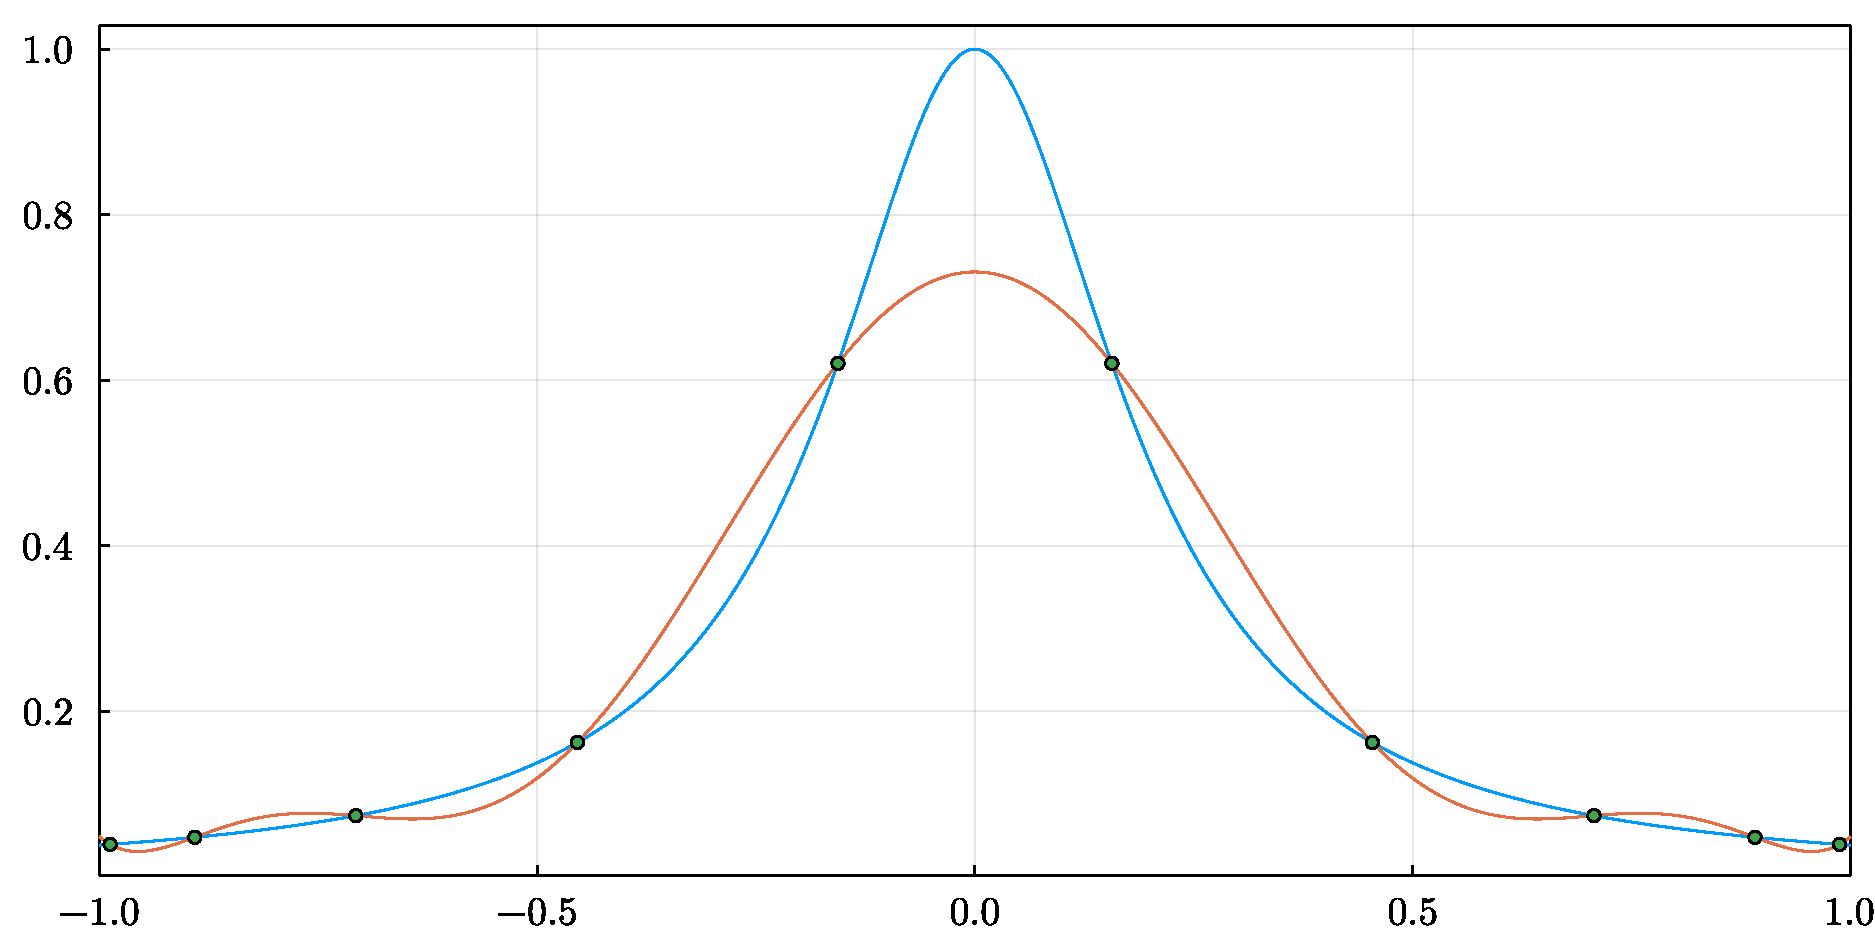
\includegraphics[width=0.49\linewidth]{figures/interpolation_cheb_runge_10.pdf}
    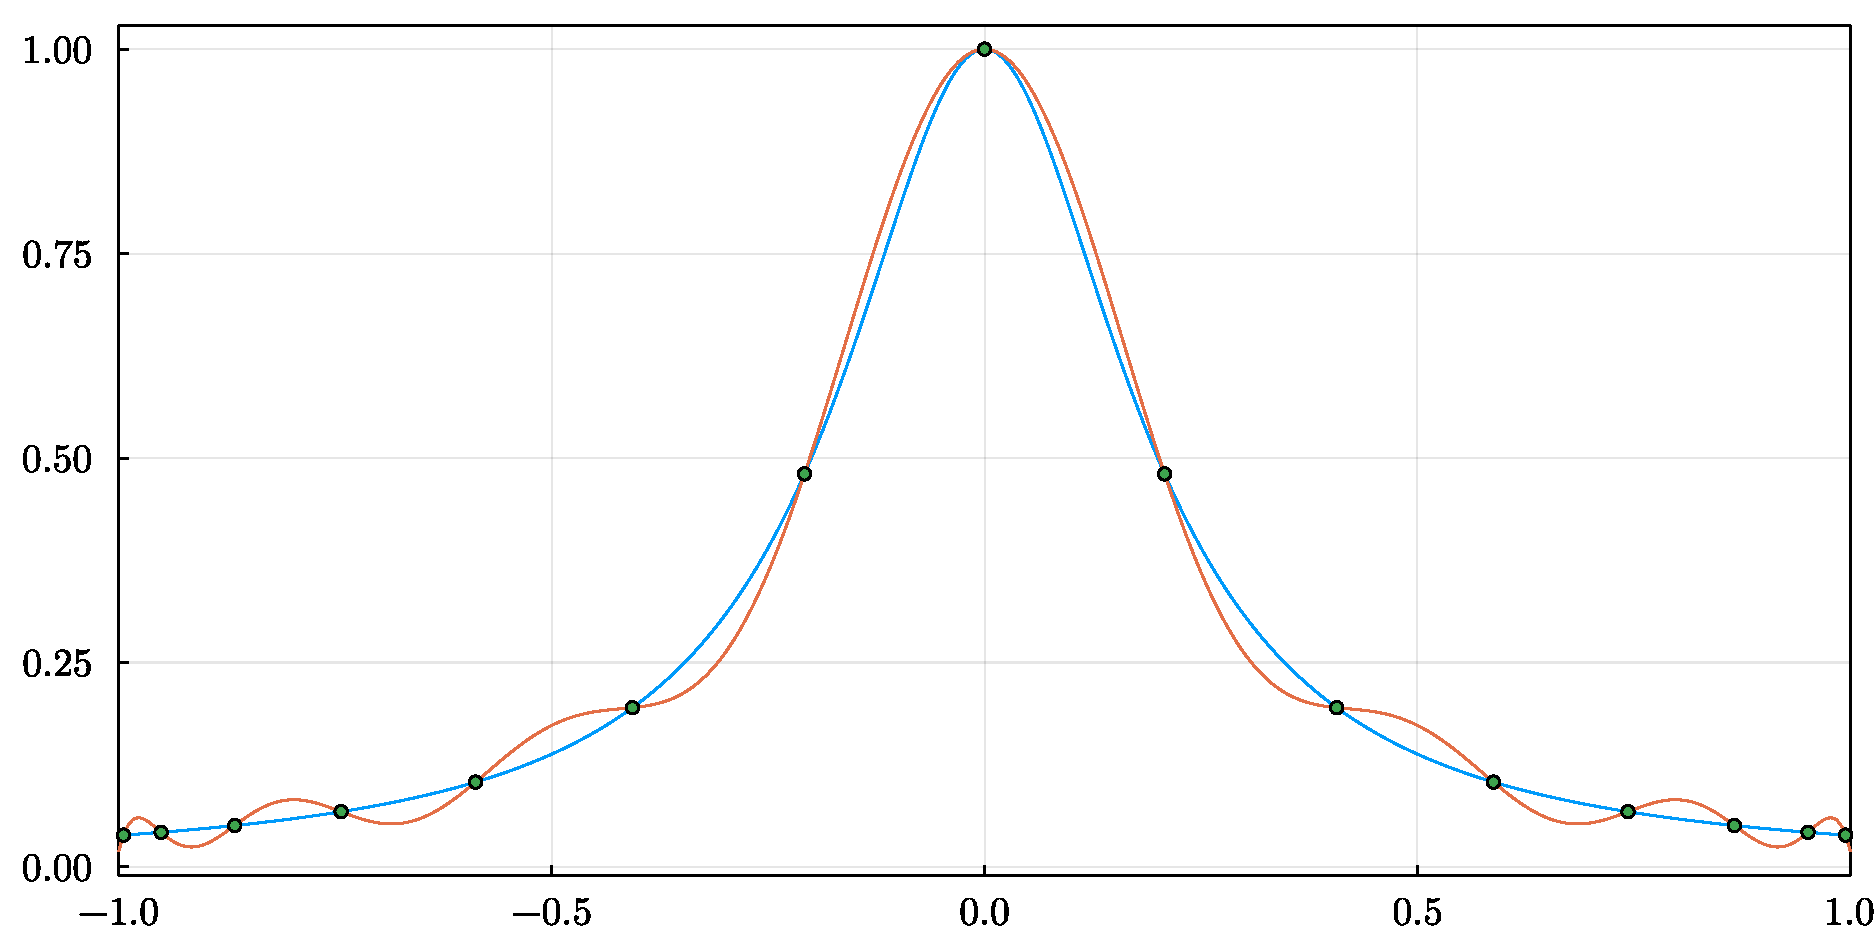
\includegraphics[width=0.49\linewidth]{figures/interpolation_cheb_runge_15.pdf}
    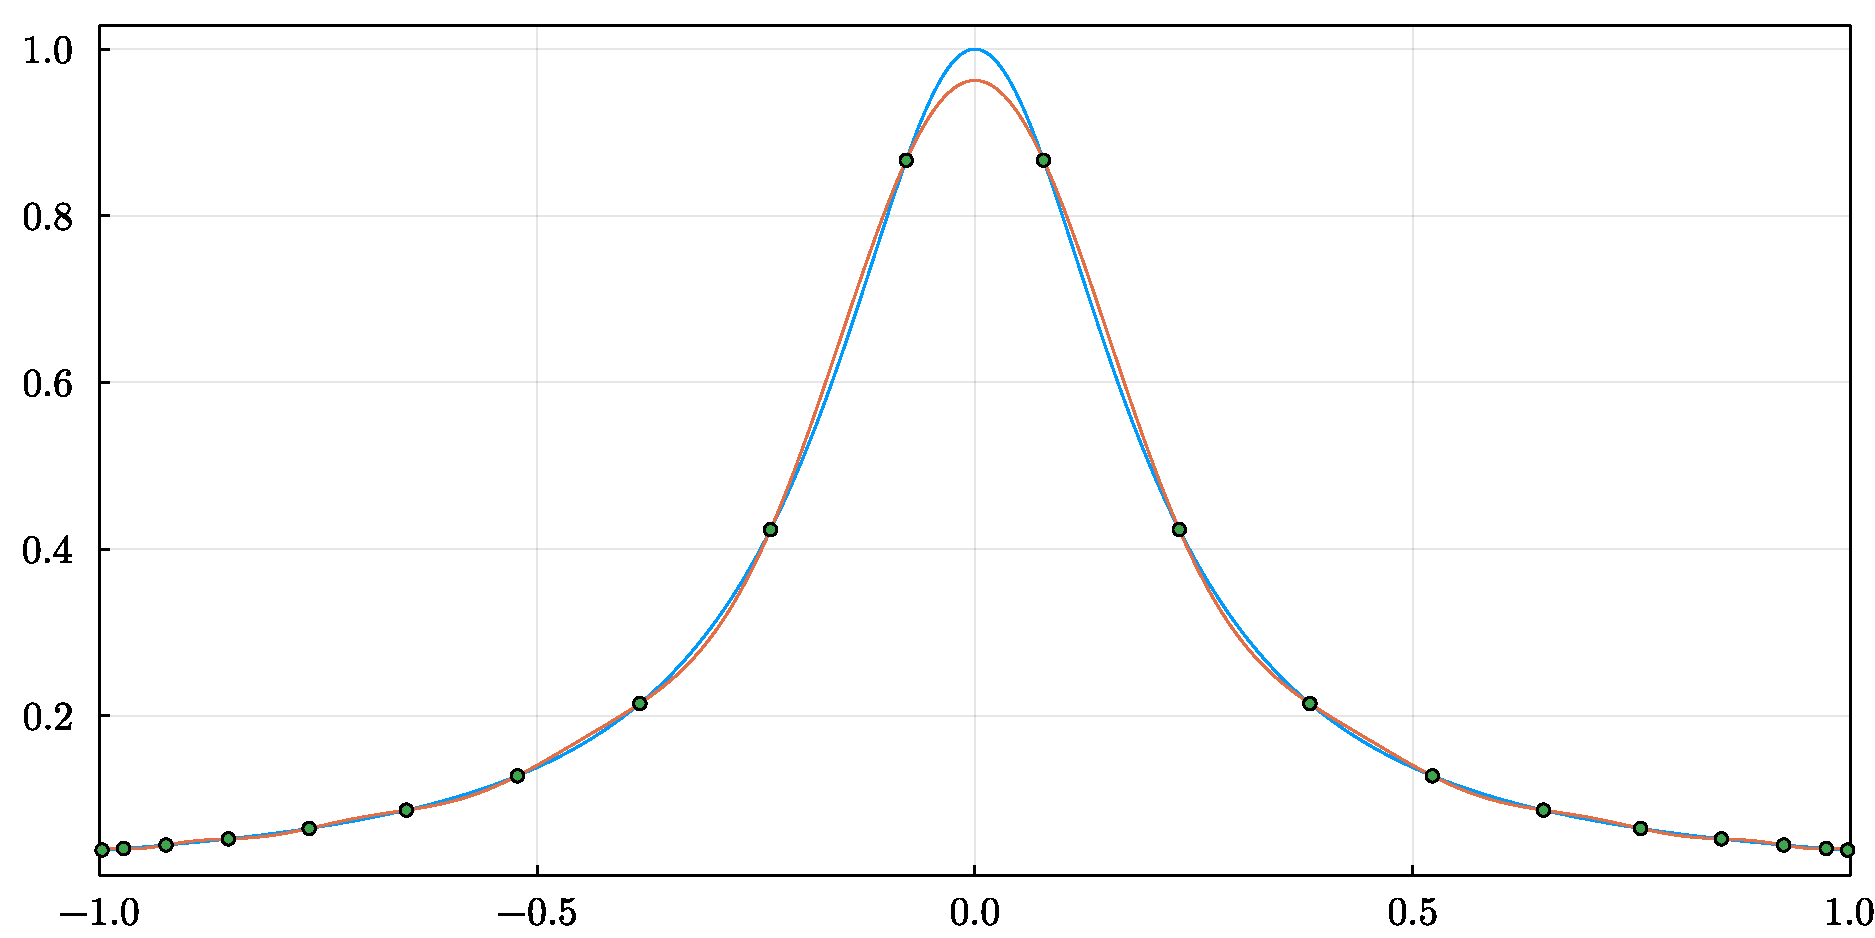
\includegraphics[width=0.49\linewidth]{figures/interpolation_cheb_runge_20.pdf}
    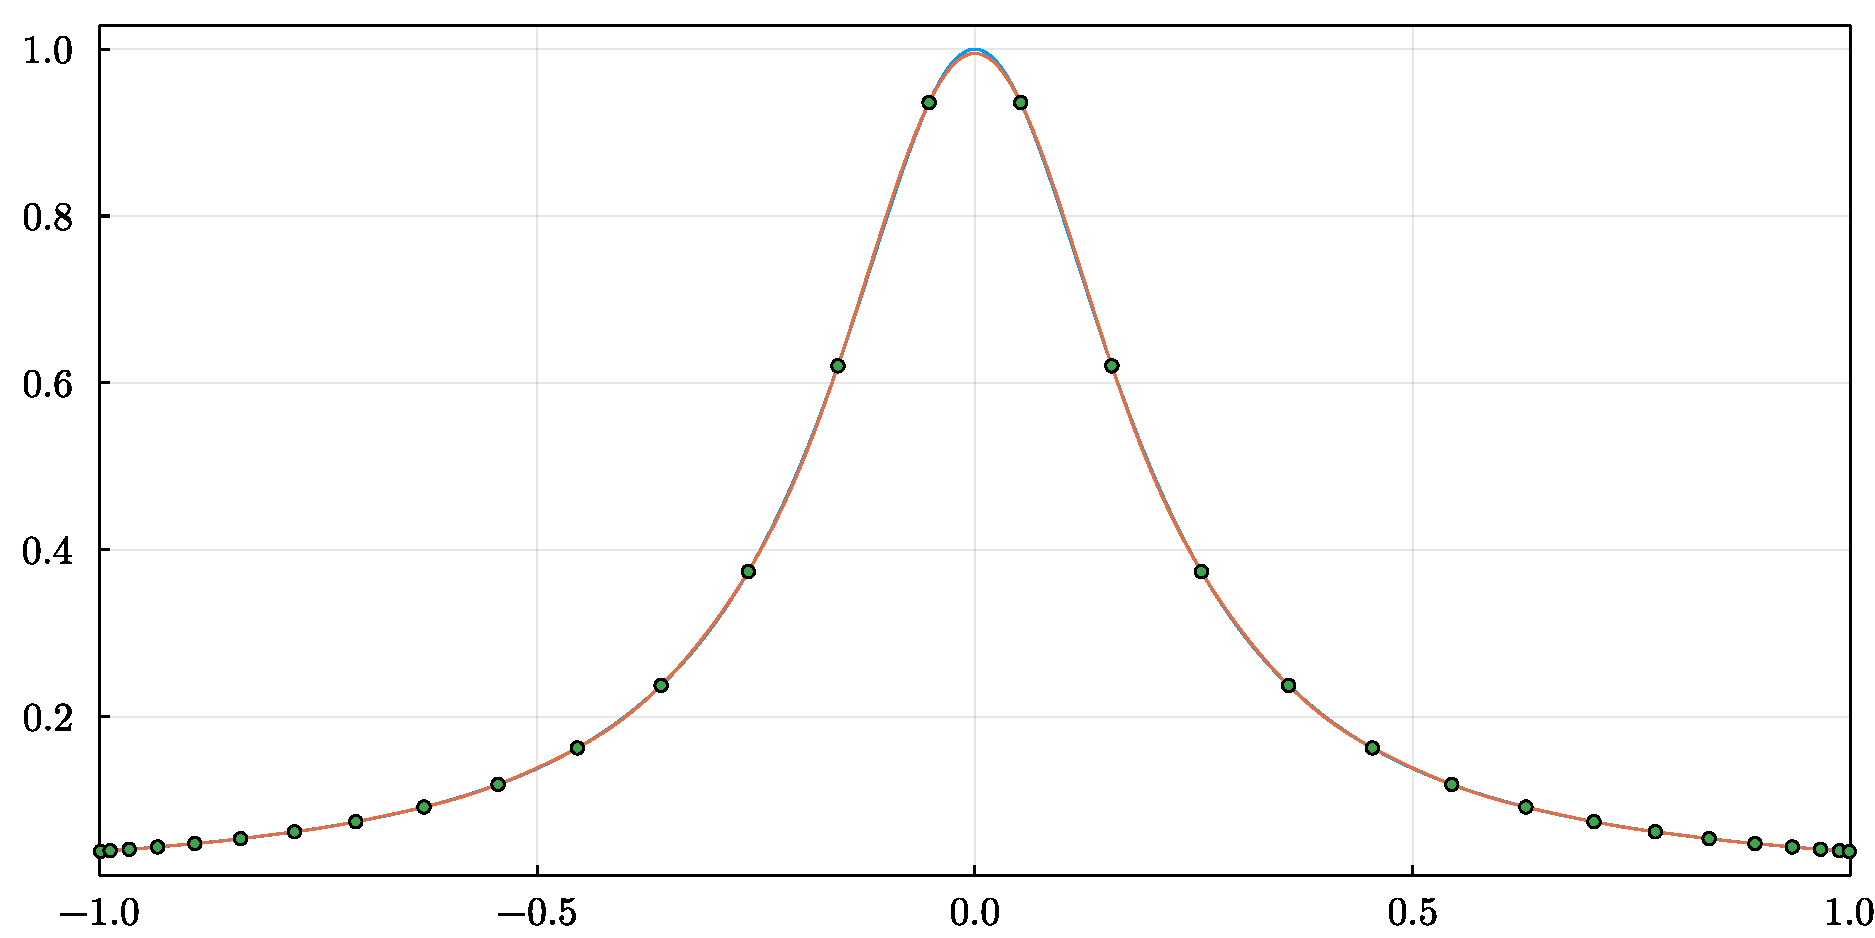
\includegraphics[width=0.49\linewidth]{figures/interpolation_cheb_runge_30.pdf}
    \label{fig:cheb_runge}
\end{figure}

\subsection{Hermite interpolation}
Hermite interpolation,
sometimes also called Hermite--Birkoff interpolation,
generalizes Lagrange interpolation to the case where,
in addition to the function values $u_0, \dotsc, u_n$,
the values of some of the derivatives are given at the interpolation nodes.
For simplicity,
we assume in this section that only the first derivative is specified.
In this case, the aim of Hermite interpolation is to find,
given data~$(x_i, u_i, u_i')$ for $i \in \{0, \dotsc, n\}$,
a polynomial~$\widehat u$ of degree at most~$2n + 1$ such that
\[
    \forall i \in \{0, \dotsc, n\}, \qquad
    \widehat u(x_i) = u_i, \qquad
    \widehat u'(x_i) = u'_i.
\]
In order to construct the interpolating polynomial,
it is useful to define the functions
\[
    \varphi_{i}(x)
    = \prod_{j=0, j\neq i}^{n} \left( \frac{x-x_j}{x_i-x_j} \right)^2,
    \qquad i = 0, \dotsc, n.
\]
The function $\varphi_i$ is the square of the usual Lagrange polynomials associated with~$x_i$,
and it satisfies
\[
    \varphi_i(x_j) = 1,
    \qquad \varphi_i'(x_i) = \sum_{j=0,j\neq i}^{n} \frac{2}{x_i - x_j},
    \qquad \forall j \neq i \qquad \varphi_i(x_j) = \varphi_i'(x_j) = 0.
\]
We consider the following ansatz for~$\widehat u$:
\[
    \widehat u(x) = \sum_{i=0}^{n} \varphi_i(x) q_i(x),
\]
where $q_i$ are polynomials to be determined of degree at most one,
so that~$\widehat u$ is of degree at most~$2n+1$.
We then require
\[
    \widehat u(x_i) = q_i(x_i), \qquad \widehat u'(x_i) = \varphi_i'(x_i) q(x_i) + q'(x_i).
\]
From the first equation, we deduce that $q_i(x_i) = u_i$,
and from the second equation we then have~$q'(x_i) = \widehat u'(x_i) - \varphi_i'(x_i) u_i$.
We conclude that the interpolating polynomial is given by
\[
    \widehat u(x) = \sum_{i=0}^{n} \varphi_i(x) \Bigl(u_i + \bigl(u_i' - \varphi_i'(x_i) u_i\bigr) (x - x_i)\Bigr).
\]
The following theorem gives an expression of the error.
\begin{theorem}
    [Hermite interpolation error]
    \label{theorem:hermite_interpolation}
    Assume that~$u\colon [a, b] \to \real$ is a function in $C^{2n+2}([a, b])$ and let~$\widehat u$
    denote the Hermite interpolation of~$u$ at the nodes~$x_0, \dotsc, x_n$.
    Then for all $x \in [a, b]$,
    there exists~$\xi = \xi(x)$ in the interval $[a, b]$ such that
    \[
        u(x) - \widehat u(x) = \frac{u^{(2n+2)}(\xi)}{(2n+2)!} (x-x_0)^2 \dotsc (x - x_n)^2.
    \]
\end{theorem}
\begin{proof}
    See~\cref{exercise:proof_hermite}.
\end{proof}

\subsection{Piecewise interpolation}
\label{sub:piecewise_interpolation}
The interpolation methods we discussed so far are in some sense global;
they aim to construct one polynomial that goes through all the data points.
This approach is attractive because the interpolant is infinitely smooth but,
as we showed, it is not always fruitful,
in particular when equidistant interpolation nodes are employed.
An alternative approach is to divide the domain in a number of small intervals,
and to perform polynomial interpolation within each interval.
Although the resulting interpolating function is usually not smooth over the full domain,
this ``local'' approach to interpolation is in general more robust.

Several methods belong in the category of piecewise interpolation.
We mention, for instance, piecewise Lagrange interpolation and cubic splines interpolation.
In this section,
we briefly describe the former method,
which is widely used in the context of the \emph{finite element method}.
Information on the latter method is available in~\cite[Section 8.7.1.]{MR2265914}.

For simplicity, we illustrate the method in dimension 1,
but piecewise Lagrange interpolation can be extended to several dimensions.
Assume that we wish to approximate a function~$u\colon [a, b] \to \real$.
We consider a subdivision $a = x_0 < x_1 < \dotsc < x_n = b$ of the interval $[a, b]$
and let~$h$ denote the maximum spacing:
\[
    h = \max_{i \in \{0, \dotsc, n-1\}} \abs{x_{i+1} - x_i}.
\]
Within each subinterval $I_i = [x_i, x_{i+1}]$,
we consider a further subdivision
\[
    x_i = x_i^{(0)} < x_i^{(1)} < \dotsc < x_i^{(m)} = x_{i+1},
\]
where the nodes $x_i^{(0)}, \dotsc, x_i^{(m)}$ are equally spaced with distance $h/m$.
The idea of piecewise Lagrange interpolation is to calculate,
for each interval $I_i$ in the partition,
the interpolating polynomial~$p_i$ at the nodes $x_i^{(0)}, \dotsc, x_i^{(m)}$.
The interpolant is then defined as
\begin{equation}
    \label{eq:piecewise_interpolation}
    \widehat u(x) = p_{\iota}(x),
\end{equation}
where $\iota = \iota(x)$ is the index of the interval to which $x$ belongs.
Since $x_i^{(m)} = x_{i+1} = x_{i+1}^{(0)}$,
the interpolant defined by~\eqref{eq:piecewise_interpolation} is continuous.
If the function $u$ belongs to $C^{m+1}([a, b])$,
then by~\cref{corollary:interpolation_error} the interpolation error within each subinterval may be bounded from above as follows:
\begin{equation}
    \label{eq:error_estimate_piecewise_interpolation}
    \sup_{x \in I_i} \abs{u(x) - \widehat u(x)} \leq \frac{ C_{m+1} (h/m)^{m+1}}{4(m + 1)},
    \qquad C_{m+1} := \sup_{x \in [a, b]} \abs{u^{(m+1)}(x)},
\end{equation}
and so we deduce
\begin{equation*}
    \sup_{x \in [a, b]} \abs{u(x) - \widehat u(x)} \leq C h^{m+1},
\end{equation*}
for an appropriate constant~$C$ independent of $h$.
This equation shows that the error is guaranteed to decrease to~0 in the limit as $h \to \infty$.
In practice, the number $m$ of interpolation nodes within each interval can be small.
% Several integration methods presented~\cref{cha:quadrature} are related to piecewise interpolation.

\section{Approximation}
In this section,
we focus on the subject of \emph{approximation},
both of discrete data points and of continuous functions.
We begin, in \cref{sub:polynomial_regression} with a discussion of least squares approximation for data points,
and in \cref{sub:mean_square_approximation} we focus on function approximation in the mean square sense.

\subsection{Least squares approximation of data points}
\label{sub:polynomial_regression}
Consider $n + 1$ distinct $x$ values $x_0 < \dotsc < x_n$,
and suppose that we know the values $u_0, \dotsc, u_n$ taken by an unknown function $u$ when evaluated at these points.
We wish to approximate the function~$u$ by a function of the form
\begin{equation}
    \label{eq:expansion_approx}
    \widehat u(x) = \sum_{i=0}^{m} \alpha_i \varphi_i(x) \in \Span \{ \varphi_0, \dotsc, \varphi_m \},
\end{equation}
for some $m < n$.
In many cases of practical interest,
the basis functions $\varphi_0, \dotsc, \varphi_m$ are polynomials.
In contrast with interpolation,
here we seek a function $\widehat u$ in a finite-dimensional function space of dimension~$m$ strictly lower than the number of data points.
In order for~$\widehat u$ to be a good approximation,
we wish to find coefficients $\alpha_0, \dotsc, \alpha_m$ such that
the following linear system is approximately satisfied.
\[
    \mat A \vect \alpha :=
    \begin{pmatrix}
        \varphi_0(x_0) & \varphi_1(x_0) & \hdots & \varphi_m(x_0) \\
        \varphi_0(x_1) & \varphi_1(x_1) & \hdots & \varphi_m(x_1) \\
        \varphi_0(x_2) & \varphi_1(x_2) & \hdots & \varphi_m(x_2) \\
        \vdots & \vdots & & \vdots \\
        \varphi_0(x_{n-2}) & \varphi_1(x_{n-2}) & \hdots & \varphi_m(x_{n-2}) \\
        \varphi_0(x_{n-1}) & \varphi_1(x_{n-1}) & \hdots & \varphi_m(x_{n-1}) \\
        \varphi_0(x_n) & \varphi_1(x_n) & \hdots & \varphi_m(x_n)
    \end{pmatrix}
    \begin{pmatrix}
        \alpha_0 \\
        \alpha_1 \\
        \vdots \\
        \alpha_m
    \end{pmatrix}
    \approx
    \begin{pmatrix}
        u_0 \\
        u_1 \\
        u_2 \\
        \vdots \\
        u_{n-2} \\
        u_{n-1} \\
        u_n
    \end{pmatrix} =: \vect b.
\]
In general,
since the matrix on the left-hand side has more lines than columns,
there does not exist an exact solution to this equation.
In order to find an approximate solution,
a natural approach is to find coefficients $\alpha_0, \dotsc, \alpha_m$ such that
the residual vector $\vect r = \mat A \vect \alpha - \vect b$ is small in some vector norm.
A particularly popular approach,
known as least squares approximation,
is to minimize the Euclidean norm of~$\vect r$ or,
equivalently, the square of the Euclidean norm:
\[
    \norm{\vect r}^2 = \sum_{i=0}^{n} \abs[big]{u_i - \widehat u(x_i)}^2 = \sum_{i=0}^{n} \left( u_i - \sum_{j=0}^{m} \alpha_j \varphi_j(x_i) \right)^2.
\]
Let us denote the right-hand side of this equation by~$J(\vect \alpha)$,
which we view as a function of the vector of coefficients $\vect a$.
A necessary condition for~$\vect a_*$ to be a minimizer is that $\nabla J(\vect \alpha_*) = 0$.
The gradient of $J$,
written as a column vector, is given by
\begin{align*}
    \nabla J(\vect \alpha)
    &= \nabla \Bigl( (\mat A \vect \alpha - \vect b)^\t (\mat A \vect \alpha - \vect b) \Bigr) \\
    &= \nabla \Bigl( \vect \alpha^\t (\mat A^\t \mat A) \vect \alpha - \vect b \mat A  \vect \alpha - \vect \alpha^\t \mat A^\t \vect b + \vect b^\t \vect b) \Bigr) \\
    &= 2 (\mat A^\t \mat A) \vect \alpha - 2 \mat A^\t \vect b.
\end{align*}
We deduce that $\vect \alpha_*$ solves the linear system
\begin{equation}
    \label{eq:normal_equation}
    \mat A^\t \mat A \vect \alpha_* = \mat A^\t \vect b,
\end{equation}
where the matrix on the left-hand side is given by:
\[
    \mat A^\t \mat A :=
    \begin{pmatrix}
        \sum_{i=0}^{n} \varphi_0(x_i) \varphi_0(x_i) & \sum_{i=0}^{n} \varphi_0(x_i) \varphi_1(x_i) & \hdots & \sum_{i=0}^{n} \varphi_0(x_i) \varphi_m(x_i) \\
        \sum_{i=0}^{n} \varphi_1(x_i) \varphi_0(x_i) & \sum_{i=0}^{n} \varphi_1(x_i) \varphi_1(x_i) & \hdots & \sum_{i=0}^{n} \varphi_1(x_i) \varphi_m(x_i) \\
        \vdots & \vdots & & \vdots \\
        \sum_{i=0}^{n} \varphi_m(x_i) \varphi_0(x_i) & \sum_{i=0}^{n} \varphi_m(x_i) \varphi_1(x_i) & \hdots & \sum_{i=0}^{n} \varphi_m(x_i) \varphi_m(x_i)
    \end{pmatrix}.
\]
Equation~\eqref{eq:normal_equation} is a system of~$m$ equations with $m$ unknowns,
which admits a unique solution provided that $\mat A^\t \mat A$ is full rank or,
equivalently, the columns of~$\mat A$ are linearly independent.
The linear equations~\eqref{eq:normal_equation} are known as the \emph{normal equations}.
As a side note,
we mention that
the solution $\vect \alpha_* = (\mat A^\t \mat A)^{-1} \mat A^\t \vect b$
coincides with the maximum likelihood estimator for $\alpha$ under the assumption that the data is generated according to
$u_i = u(x_i) + \varepsilon_i$, for some function $u \in \Span \{\varphi_0, \dotsc, \varphi_m\}$
and random noise $\varepsilon_i \sim \mathcal N(0, 1)$.

\begin{remark}
From equation~\eqref{eq:normal_equation} we deduce that
\[
    \mat A \vect \alpha_* = \mat A (\mat A^\t \mat A)^{-1} \mat A^\t \vect b.
\]
The matrix~$\Pi_{\mat A} := \mat A (\mat A^\t \mat A)^{-1} \mat A^\t$ on the right-hand side is the orthogonal projection operator onto $\col(\mat A) \subset \real^n$,
the subspace spanned by the columns of~$\mat A$.
Indeed, it holds that $\Pi_{\mat A}^2 = \Pi_{\mat A}$,
which is the defining property of a projection operator.
\end{remark}

To conclude this section,
we note that the matrix $\mat A^{+} = (\mat A^\t \mat A)^{-1} \mat A^\t$ is a left inverse of the matrix $\mat A$,
because $\mat A^+ \mat A = \mat I$.
It is also called the Moore--Penrose inverse or pseudoinverse of the matrix~$\mat A$,
which generalizes the usual inverse matrix.
In Julia, the backslash operator silently uses the Moore--Penrose inverse when employed with a rectangular matrix.
Therefore, solving the normal equations~\eqref{eq:normal_equation} can be achieved by just writing \julia{α = A\b}.

\subsection{Mean square approximation of functions}
\label{sub:mean_square_approximation}
The approach described in~\cref{sub:polynomial_regression} can be generalized to the setting where the actual function~$u$,
rather than just discrete evaluations of it, is available.
In this section, we seek an approximation of the form~\eqref{eq:expansion_approx}
such that the error $\widehat u(x) - u(x)$, measured in some function norm,
is minimized.
Of course, the solution to this minimization problem depends in general on the norm employed,
and may in some cases not even be unique.
Instead of specifying a particular norm,
as done in \cref{sub:polynomial_regression},
in this section we retain some generality and assume only that the norm is induced by an inner product on the space of real-valued continuous functions:
\begin{equation}
    \label{eq:inner_product_approx}
    \ip{\placeholder,\placeholder} \colon C([a,b]) \times C([a, b]) \to \real.
\end{equation}
In other words,
we seek to minimize
\[
    J(\vect \alpha) := \norm{\widehat u - u}^2 = \ip{\widehat u - u, \widehat u - u}.
\]
This is again a function of the $m+1$ variables $\alpha_0, \dotsc, \alpha_m$.
Before calculating its gradient,
we rewrite the function $J(\vect \alpha)$ in a simpler form:
\begin{align*}
    J(\vect \alpha)
    &= \ip*{u - \sum_{j=0}^{m} \alpha_j \varphi_j,u - \sum_{k=0}^{m} \alpha_k \varphi_k} \\
    &= \sum_{j=0}^{m} \sum_{k=0}^{m} \alpha_j \alpha_k \ip{\varphi_j,\varphi_k}- 2 \sum_{j=0}^{m} \alpha_j \ip{u,\varphi_j} - \ip{u,u}
    = \vect \alpha^\t \mat G \vect \alpha - 2 \vect b^\t \vect \alpha - \ip{u,u},
\end{align*}
where we introduced
\begin{equation}
    \label{eq:approx_matrix_m}
    \mat G :=
    \begin{pmatrix}
        \ip{\varphi_0, \varphi_0} & \ip{\varphi_0, \varphi_1} & \hdots & \ip{\varphi_0, \varphi_m} \\
        \ip{\varphi_1, \varphi_0} & \ip{\varphi_1, \varphi_1} & \hdots & \ip{\varphi_1, \varphi_m} \\
        \vdots & \vdots & & \vdots \\
        \ip{\varphi_m, \varphi_0} & \ip{\varphi_m, \varphi_1} & \hdots & \ip{\varphi_m, \varphi_m}
    \end{pmatrix},
    \qquad
    \vect b :=
    \begin{pmatrix}
        \ip{u, \varphi_0} \\
        \ip{u, \varphi_1} \\
        \vdots \\
        \ip{u, \varphi_m} \\
    \end{pmatrix}.
\end{equation}
Employing the same approach as in the previous section,
we then obtain $\nabla J(\vect \alpha) = \mat G \vect \alpha - \vect b$,
and so the minimizer of $J(\vect \alpha)$ is the solution to the equation
\begin{equation}
    \label{eq:normaal_continuous}
    \mat G \vect \alpha_* = \vect b.
\end{equation}
The matrix $\mat G$,
known as the \emph{Gram matrix},
is positive semi-definite and nonsingular provided that the basis functions are linearly independent,
see~\cref{exercise:matrix_approx}.
Therefore, the solution $\vect \alpha_*$ exists and is unique.
In addition, since the Hessian of~$J$ is equal to~$\mat G$,
the vector~$\vect \alpha_*$ is indeed a minimizer.
Note that if~$\ip{\placeholder,\placeholder}$ is defined as a finite sum of the form
\begin{equation}
    \label{eq:inner_finite}
    \ip{f, g} = \sum_{i=0}^{n} f(x_i) g(x_i),
\end{equation}
then~\eqref{eq:normaal_continuous} coincides with the normal equations~\eqref{eq:normal_equation} from the previous section.
We remark that~\eqref{eq:inner_finite} is in fact not an inner product on the space of continuous functions,
but it is an inner product on the space of polynomials of degree less than or equal to~$n$.

In practice, the matrix and right-hand side of the linear system~\eqref{eq:normaal_continuous} can usually not be calculated exactly,
because the inner product~$\ip{\placeholder,\placeholder}$ is defined through an integral; see~\eqref{eq:ip_weighted} in the next section.

\begin{remark}
    Rewriting the normal equations~\eqref{eq:normaal_continuous} in terms of~$\widehat u$
    we obtain
    \begin{align*}
        \ip{\widehat u - u,\varphi_0} &= 0,
        \qquad
        \dots, \qquad
        \ip{\widehat u - u,\varphi_m} &= 0.
    \end{align*}
    Therefore, the optimal approximation $\widehat u \in \Span \{ \varphi_0, \dotsc, \varphi_m \}$ satisfies
    \[
        \forall v \in \Span \{ \varphi_0, \dotsc, \varphi_m \}, \qquad \ip{\widehat u - u, v} = 0.
    \]
    This shows that the optimal approximation $\widehat u$,
    in the sense of the norm~$\norm{\placeholder}$,
    is the orthogonal projection of~$u$ onto $\Span \{ \varphi_0, \dotsc, \varphi_m \}$.
\end{remark}
\subsection{Orthogonal polynomials}
The Gram matrix~$\mat G$ in~\eqref{eq:normaal_continuous} is equal to the identity matrix when the basis functions are orthonormal for the inner product considered.
In this case, the solution to the linear system is
\[
    \alpha_i = \ip{u, \varphi_i}, \qquad i = 0, \dotsc, m,
\]
and so the best approximation~$\widehat u$ (for the norm induced by the inner product considered!) is simply given by
\[
    \widehat u = \sum_{i=0}^{m} \ip{u, \varphi_i} \varphi_i.
\]
The coefficients $\ip{u, \varphi_i}$ of the basis functions in this expansion are called \emph{Fourier coefficients}.
% and this equation shows that the best approximation is an orthogonal projection.
Given a finite dimensional subspace~$\mathcal S$ of the space of continuous functions,
an orthonormal basis can be constructed via the Gram--Schmidt process.
In this section, we focus on the particular case where $\mathcal S = \poly(n)$
-- the subspace of polynomials of degree less than or equal to $n$.
Another widely used approach,
which we do not explore in this course,
is to use trigonometric basis functions.
We also assume that the inner product~\eqref{eq:inner_product_approx} is of the form
\begin{equation}
    \label{eq:ip_weighted}
    \ip{f,g}
    = \int_{a}^{b} f(x) g(x) w(x) \, \d x,
\end{equation}
where $w(x)$ is a given nonnegative weight function such that
\[
    \int_{a}^{b} w(x) \, \d x > 0.
\]
Let $\varphi_0(x), \varphi_1(x), \varphi_2(x) \dotsc$ denote the orthonormal polynomials obtained by applying the Gram--Schmidt procedure to the monomials $1, x, x^2, \dotsc$.
These depend in general on the weight~$w(x)$ and on the interval~$[a, b]$.
A few of the popular classes of orthogonal polynomials are presented in the table below:
\begin{center}
    \def\arraystretch{1.5}
    \begin{tabular}{|c|c|c|}
        \hline
        \textbf{Name} & $w(x)$  & $[a, b]$ \\ \hline
        Legendre & $1$  & $[-1, 1]$ \\ \hline
        Chebyshev & $\frac{1}{\sqrt{1 - x^2}}$  & $(-1, 1)$ \\ \hline
        Hermite & $\exp \left( - \frac{x^2}{2} \right)$  & $[-\infty, \infty]$ \\ \hline
        Laguerre & $\e^{-x}$  & $[0, \infty]$ \\ \hline
    \end{tabular}
\end{center}

Orthogonal polynomials have a rich structure,
and in the rest of this section we prove some of their common properties,
one of which will be very useful in the context of numerical integration in~\cref{cha:quadrature}.
We begin by showing that
orthogonal polynomials have distinct real roots.
\begin{proposition}
    \label{proposition:distinct_roots}
    Assume for simplicity that $w(x) > 0$ for all $x \in [a, b]$,
    and let $\varphi_0, \varphi_1, \dotsc$ denote orthonormal polynomials of increasing degree for the inner product~\eqref{eq:ip_weighted}.
    Then for all $n \in \nat$,
    the polynomial $\varphi_n$ has~$n$ distinct roots in the open interval $(a, b)$.
\end{proposition}
\begin{proof}
    Reasoning by contradiction,
    we assume that~$\varphi_n$ changes sign at only $k < n$ points of the open interval~$(a, b)$,
    which we denote by $x_1, \dotsc, x_k$.
    Then
    \[
        \varphi_n(x) \times (x - x_0) (x - x_1) \dotsc (x - x_k)
    \]
    is either everywhere nonnegative or everywhere nonpositive over $[a, b]$
    But then
    \[
        \int_{a}^{b} \varphi_n(x) \times (x - x_1)  \dotsc (x - x_k) \, w(x) \, \d x
    \]
    is nonzero,
    which is a contradiction because the product $(x-x_1) \dotsc (x-x_k)$ is a polynomial of degree~$k$,
    which is orthogonal to $\varphi_n$ by assumption.
    Indeed, being orthogonal to~$\varphi_0, \dotsc, \varphi_{n-1}$,
    the polynomial $\varphi_n$ is also orthogonal to any linear combination of these polynomials.
\end{proof}

Next, we show that orthogonal polynomials satisfy a three-term recurrence relation.
\begin{proposition}
    \label{proposition:three_term_recurrence}
    Assume that $\varphi_0, \varphi_1, \dotsc$ are orthonormal polynomials
    for some inner product of the form~\eqref{eq:ip_weighted} such that $\varphi_i$ is of degree~$i$.
    Then
    \begin{equation}
        \label{eq:recurrence_ortho}
        \forall n \in \{1, 2, \dotsc\}, \qquad
        \alpha_{n+1} \varphi_{n+1} (x) = (x - \beta_n) \varphi_n(x) - \alpha_{n} \varphi_{n-1}(x),
    \end{equation}
    where
    \[
        \alpha_n = \ip[big]{x \varphi_n, \varphi_{n-1}},
        \qquad \beta_n = \ip[big]{x \varphi_n, \varphi_{n}}.
    \]
    In addition, $\alpha_1 \varphi_{1} (x) = (x - \beta_0) \varphi_0(x)$.
\end{proposition}
\begin{proof}
    Since $x \varphi_n(x)$ is a polynomial of degree $n+1$,
    it may be decomposed as
    \begin{equation}
        \label{eq:expansion_times_x}
        x \varphi_n(x) = \sum_{i=0}^{n+1} \gamma_{n,i} \varphi_i(x).
    \end{equation}
    Taking the inner product of both sides of this equation with~$\varphi_i$
    and employing the orthonormality assumption,
    we obtain an expression for the coefficients:
    \[
        \gamma_{n,i} = \ip[big]{x \varphi_n, \varphi_i}.
    \]
    From the expression~\eqref{eq:ip_weighted} of the inner product,
    it is clear that $\ip[big]{x \varphi_n, \varphi_i} = \ip[big]{\varphi_n, x\varphi_i}$.
    Since~$x \varphi_i$ is a polynomial of degree $i+1$ and $\varphi_n$ is orthogonal to all polynomials of degree strictly less than~$n$,
    we deduce that $\gamma_{n,i} = 0$ if~$i < n-1$.
    Consequently, we can rewrite the right-hand side of~\eqref{eq:expansion_times_x} as a sum involving only three terms
    \begin{equation}
        \label{eq:expansion_times_x_good}
        x \varphi_n(x) =  \ip[big]{x \varphi_n, \varphi_{n-1}} \varphi_{n-1}(x) + \ip[big]{x \varphi_n, \varphi_{n}} \varphi_{n}(x) + \ip[big]{x \varphi_n, \varphi_{n+1}} \varphi_{n+1}(x).
    \end{equation}
    Since $\ip[big]{x \varphi_n, \varphi_{n+1}} = \ip[big]{x \varphi_{n+1}, \varphi_{n}}$,
    we obtain the statement after rearranging.
\end{proof}
\begin{remark}
    Notice that the polynomials in~\eqref{proposition:three_term_recurrence} are orthonormal by assumption,
    and so the coefficient~$\alpha_{n+1}$ is just a normalization constant.
    We deduce that
    \[
        \varphi_{n+1} (x) = \frac{(x - \beta_n) \varphi_n(x) - \alpha_{n} \varphi_{n-1}(x)}{\norm{(x - \beta_n) \varphi_n(x) - \alpha_{n} \varphi_{n-1}(x)}},
    \]
    which enables to calculate the orthogonal polynomials recursively.
\end{remark}

\subsection{Orthogonal polynomials and numerical integration: an introduction~\moreinfo}
\label{sub:orthogonal_integration}
Equation~\eqref{eq:expansion_times_x_good} may be rewritten in matrix form as follows:
\[
    \begin{pmatrix}
        x \varphi_0(x) \\
        x \varphi_1(x) \\
        x \varphi_2(x) \\
        \vdots \\
        x \varphi_{m-1}(x) \\
        x \varphi_m(x)
    \end{pmatrix}
    =
    \begin{pmatrix}
        \beta_0 & \alpha_1 \\
        \alpha_1 & \beta_1 & \alpha_2 \\
                 & \alpha_2 & \beta_2 & \alpha_3 \\
                 & & \ddots & \ddots & \ddots \\
                 & & & \alpha_{m-1} & \beta_{m-1} & \alpha_m \\
                 & & & & \alpha_m & \beta_m
    \end{pmatrix}
    \begin{pmatrix}
        \varphi_0(x) \\
        \varphi_1(x) \\
        \varphi_2(x) \\
        \vdots \\
        \varphi_{m-1}(x) \\
        \varphi_m(x)
    \end{pmatrix}
    +
    \begin{pmatrix}
        0 \\
        0 \\
        0 \\
        \vdots \\
        0 \\
        \alpha_{m+1} \varphi_{m+1}(x)
    \end{pmatrix}.
\]
Let $\mat T$ denote the matrix on the left-hand side of this equation,
and let $r_0, \dotsc, r_{m}$ denote the roots of~$\varphi_{m+1}$.
By~\cref{proposition:distinct_roots},
these are distinct and all belong to the interval~$(a, b)$.
But now notice that
\[
    \forall r \in \Bigl\{ r_0, \dotsc, r_m \Bigr\}, \qquad
    \begin{pmatrix}
        r \varphi_0(r) \\
        r \varphi_1(r) \\
        \vdots \\
        r \varphi_{m-1}(r) \\
        r \varphi_m(r)
    \end{pmatrix}
    =
    \begin{pmatrix}
        \beta_0 & \alpha_1 \\
        \alpha_1 & \beta_1 & \alpha_2 \\
                 & \ddots & \ddots & \ddots \\
                 & & \alpha_{m-1} & \beta_{m-1} & \alpha_m \\
                 & & & \alpha_m & \beta_m
    \end{pmatrix}
    \begin{pmatrix}
        \varphi_0(r) \\
        \varphi_1(r) \\
        \vdots \\
        \varphi_{m-1}(r) \\
        \varphi_m(r)
    \end{pmatrix}.
\]
In other words,
for any root $r$ of~$\varphi_{m+1}$,
the vector $\begin{pmatrix} \varphi_0(r) & \hdots & \varphi_m(r) \end{pmatrix}^\t$
is an eigenvector of the matrix~$\mat T$,
with associated eigenvalue equal to~$r$.
Since~$\mat T$ is a symmetric matrix,
the eigenvectors associated to distinct eigenvalues are orthogonal for the Euclidean inner product of~$\real^{m+1}$,
so given that the eigenvalues of~$\mat T$ are distinct,
we deduce that
\begin{equation}
    \label{eq:orthogonality}
    \forall i \neq j, \qquad
    \sum_{i=0}^{m} \varphi_i(r_i) \varphi_i(r_j) = 0.
\end{equation}
Let us construct the matrix
\[
    \mat P =
    \begin{pmatrix}
        \varphi_0(r_0) & \varphi_1(r_0) & \hdots & \varphi_m(r_0) \\
        \varphi_0(r_1) & \varphi_1(r_1) & \hdots & \varphi_m(r_1) \\
        \varphi_0(r_2) & \varphi_1(r_2) & \hdots & \varphi_m(r_2) \\
        \vdots & \vdots & \hdots & \vdots \\
        \varphi_0(r_m) & \varphi_1(r_m) & \hdots & \varphi_m(r_m)
    \end{pmatrix}.
\]
Equation~\eqref{eq:orthogonality} indicates that the lines of~$\mat P$ are orthogonal,
and so the matrix~$\mat D = \mat P \mat P^\t$ is diagonal with elements given by
\[
    d_{ii} = \sum_{j=0}^{m} \abs{\varphi_j(r_i)}^2,
    \qquad i = 0, \dotsc, m.
\]
(Here we start counting the lines from 0 for convenience.)
Since $\mat P \mat P^\t \mat D^{-1} = \mat I$,
we deduce that the inverse of~$\mat P$ is given by $\mat P^{-1} = \mat P^\t \mat D^{-1}$.
Consequently,
\[
    \mat P^\t \mat D^{-1} \mat P = \mat P^{-1} \mat P = \mat I,
\]
which means that the polynomials~$\varphi_1, \dotsc, \varphi_m$ are orthogonal for the inner product
\begin{align*}
    \ip{\placeholder, \placeholder}_{m+1} \colon& \poly(m) \times \poly(m) \to \real; \\
                              &(p, q) \mapsto \vect \sum_{i=0}^{m} \frac{p(r_i) q(r_i)}{d_{ii}}.
\end{align*}
We have thus shown that,
if~$\varphi_0, \varphi_1, \varphi_2$ are a family of orthonormal polynomials for an inner product~$\ip{\placeholder,\placeholder}$,
then they are also orthonormal for the inner product~$\ip{\placeholder,\placeholder}_{m+1}$.
Consequently, it holds that
\begin{equation}
    \label{eq:orthogonality_equivalence}
    \forall (p, q) \in \poly(m) \times \poly(m), \qquad
    \ip{p,q} = \ip{p, q}_{m+1},
\end{equation}
Indeed, denoting by $p = \alpha_0 \varphi_0 + \dotsb + \alpha_m \varphi_m$ and $q = \beta_0 \varphi_0 + \dotsb + \beta_m \varphi_m$ the expansions of the polynomials~$p$ and~$q$
in the orthonormal basis,
we have
\begin{align*}
    \ip{p, q}
    &= \ip{\alpha_0 \varphi_0 + \dotsb + \alpha_m \varphi_m,\beta_0 \varphi_0 + \dotsb + \beta_m \varphi_m} \\
    &= \sum_{i=0}^{m} \sum_{j=0}^{m} \alpha_i \beta_j \ip{\varphi_i, \varphi_j}
    = \alpha_0 \beta_0 + \dotsb + \alpha_m \beta_m
    = \sum_{i=0}^{m} \sum_{j=0}^{m} \alpha_i \beta_j \ip{\varphi_i, \varphi_j}_{m+1} \\
    & = \ip{\alpha_0 \varphi_0 + \dotsb + \alpha_m \varphi_m,\beta_0 \varphi_0 + \dotsb + \beta_m \varphi_m}_{m+1} = \ip{p,q}_{m+1}.
\end{align*}
We have thus shown the following result.
Since~$m$ was arbitrary in the previous reasoning,
we add a superscript to indicate when the quantities involved depend on~$m$.
\begin{theorem}
    Orthonormal polynomials~$\varphi_0, \dotsc, \varphi_{m}$ for the inner product
    \[
        \ip{f, g} = \int_{a}^{b} f(x) g(x) w(x) \, \d x
    \]
    are also orthonormal for the inner product
    \[
        \ip{f,g}_{m+1} = \sum_{i=0}^{m} f\left(r^{(m+1)}_i\right) g\left(r^{(m+1)}_i\right) w^{(m+1)}_i,
    \]
    where $r^{(m+1)}_0, \dotsc, r^{(m+1)}_m$ are the roots of~$\varphi_{m+1}$ and
    the weights~$w^{(m+1)}_i$ are given by
    \[
        w^{(m+1)}_i = \frac{1}{\sum_{j=0}^{m} \left\lvert \varphi_j\left(r^{(m+1)}_i\right) \right\rvert^2}, \qquad i = 0, \dotsc, m.
    \]
\end{theorem}
Taking~$q = 1$ in~\eqref{eq:orthogonality_equivalence} and employing the definitions of~$\ip{\placeholder, \placeholder}$ and $\ip{\placeholder, \placeholder}_{m+1}$,
we have
\begin{equation}
    \label{eq:integration_formula}
    \forall p \in \poly(m),
    \qquad \int_{a}^{b} p(x) \, w(x) \, \d x
    = \sum_{i=0}^{m} p\left(r_i^{(m+1)}\right) w^{(m+1)}_i.
\end{equation}
Since the left-hand side is an integral and the right-hand side is a sum,
we have just constructed an integration formula,
which enjoys a very nice property: it is exact for polynomials of degree up to~$m$!
A formula of this type is called a \emph{quadrature formula},
with~$m+1$ \emph{nodes}~$r^{(m+1)}_0, \dotsc, r^{(m+1)}_m$ and associated \emph{weights} $w^{(m+1)}_0, \dotsc, w^{(m+1)}_m$.
Note that the nodes and weights of the quadrature depend on the weight~$w(x)$ and on the degree~$m$.

In fact, equation~\eqref{eq:integration_formula} is valid more generally than for~$p \in \poly(m)$.
Indeed, for every monomial~$x^p$ with $m \leq p \leq 2m$,
we have that
\begin{align*}
    \int_{a}^{b} x^p w(x) \, \d x
    &= \int_{a}^{b} x^{p-m} x^m  w(x) \, \d x \\
    &= \ip{x^{p-m},x^m} = \ip{x^{p-m},x^m}_{m+1}
    = \ip{x^{p},1}_{m+1} = \sum_{i=0}^{m} \left(r_i^{(m+1)}\right)^{p} w^{(m+1)}_i.
\end{align*}
Consequently, the formula~\eqref{eq:integration_formula} is exact for any monomial of degree up to $2m$,
and we conclude that, by linearity, it is also valid for any polynomials of degree up to~$2m$.

\begin{remark}
    In fact, the formula~\eqref{eq:integration_formula} is valid for polynomials of degree up to~$2m+1$.
    Indeed, using that $x^{2m+1} = \varphi_{m+1}(x) p(x) + q(x)$,
    for some polynomial~$p$ of degree~$m$ (the quotient of the polynomial division of $x^{2m+1}$ by $\varphi_{m+1}$) and some polynomial~$q$ of degree less than~$m$ (the remainder of the polynomial division),
    we have
    \begin{align*}
        \int_{a}^{b} x^{2m+1} w(x) \, \d x
        &= \int_{a}^{b} \varphi_{m+1}(x) p(x) w(x) \, \d x + \int_{a}^{b} q(x) w(x) \, \d x = 0 + \int_{a}^{b} q(x) w(x) \, \d x \\
        &= \sum_{i=0}^{m} \varphi_{m+1}\left(r_i^{(m+1)}\right) p\left(r_i^{(m+1)}\right)  w^{(m+1)}_i + \sum_{i=0}^{m} q\left(r_i^{(m+1)}\right) w^{(m+1)}_i \\
        &= \sum_{i=0}^{m} \left(r_i^{(m+1)}\right)^{2m+1} w^{(m+1)}_i,
    \end{align*}
    where we used, in the penultimate inequality,
    the fact that~$r_0^{(m+1)}, \dotsc, r_m^{(m+1)}$ are the roots of the polynomial~$\varphi_{m+1}$.
\end{remark}
We will revisit this subject in~\cref{cha:quadrature}.

\section{Exercises}
\begin{exercise}
    Find the polynomial $p(x) = ax + b$ (a straight line) that goes through the points $(x_0, u_0)$ and $(x_1, u_1)$.
\end{exercise}

\begin{exercise}
    Find the polynomial $p(x) = ax^2 + b x + c$ (a parabola) that goes through the points $(0, 1)$, $(1, 3)$ and $(2, 7)$.
\end{exercise}

\begin{exercise}
    Prove the following recurrence relation for Chebyshev polynomials:
    \[
        T_{i+1}(x) = 2 x T_i(x) - T_{i-1}(x), \qquad i = 1, 2, \dotsc.
    \]
\end{exercise}

\begin{exercise}
    \label{exercise:divided_differences}
    Show by recursion that
    \[
        [u_{0}, u_{1}, \dotsc, u_{n}] = \sum_{j=0}^{n} \frac{u_{j}}{\prod_{ k \in \{0, \dotsc, n\} \backslash \{ j\}} (x_{j} - x_{k})}.
    \]
    Deduce from this identity that
    \[
        [u_{0}, u_{1}, \dotsc, u_{n}] = [u_{\sigma_1}, u_{\sigma_2}, \dotsc, u_{\sigma_n}],
    \]
    for any permutation~$\vect \sigma$ of~$(0, 1, 2, \dotsc, n)$.
\end{exercise}

\begin{exercise}
    Using the Gregory--Newton formula,
    find an expression for
    \[
        \sum_{i=1}^{n} i^4.
    \]
\end{exercise}

\begin{exercise}
    Let $(f_0, f_1, f_2, \dotsc) = (1, 1, 2, \dotsc)$ denote the Fibonacci sequence.
    Prove that there does not exist a polynomial~$p$ such that
    \[
        \forall i \in \nat, \qquad
        f_i = p(i).
    \]
\end{exercise}

\begin{exercise}
    Using the Gregory--Newton formula,
    show that
    \begin{equation}
        \label{eq:discrete_exponential}
        \forall n \in \nat_{>0},
        \qquad 2^n = 1 + n + \frac{n^{\underline{2}}}{2!} + \frac{n^{\underline 3}}{3!} + \frac{n^{\underline 4}}{4!} + \dotsb
    \end{equation}
    \begin{remark}
        Remarkably, equation~\eqref{eq:discrete_exponential} holds in fact for \emph{any} $n \in \real_{> 0}$.
        However, showing this more general statement is beyond the scope of this course.
    \end{remark}
\end{exercise}

\begin{exercise}
    \label{exercise:proof_hermite}
    Prove~\cref{theorem:hermite_interpolation}.
\end{exercise}

\begin{exercise}
    \label{exercise:matrix_approx}
    Show that the matrix $\mat G$ in \eqref{eq:approx_matrix_m} is positive definite
    if the basis functions~$\varphi_0, \dotsc, \varphi_m$ are linearly independent.
\end{exercise}

\begin{compexercise}
    Write a Julia code for interpolating the following function using a polynomial of degree 20 over the interval $[-1, 1]$.
    \[
        f(x) = \tanh\left(\frac{x+1/2}{\varepsilon}\right) + \tanh\left(\frac{x}{\varepsilon}\right) + \tanh\left(\frac{x-1/2}{\varepsilon}\right),
        \qquad \varepsilon = .01.
    \]
    Use equidistant and then Chebyshev nodes,
    and compare the two approaches in terms of accuracy.
    Plot the function~$f$ together with the approximating polynomials.
\end{compexercise}

\begin{compexercise}
    \label{exercise:parametric_interpolation}
    We wish to use interpolation to approximate the following parametric function,
    called an \emph{epitrochoid}:
    \begin{align}
        x (\theta) &= (R + r)\cos\theta + d\cos\left(\frac{R + r}{r}\theta\right) \\
      y (\theta) &= (R + r)\sin\theta - d\sin\left(\frac{R + r}{r}\theta\right),
    \end{align}
    with $R = 5$, $r = 2$ and $d = 3$, and for $\theta \in [0, 4\pi]$.
    Write a Julia program to interpolate $x(\theta)$ and $y(\theta)$ using 40 equidistant points.
    Use the \julia{BigFloat} format in order to reduce the impact of round-off errors.
    After constructing the polynomial interpolations $\widehat x(\theta)$ and $\widehat y(\theta)$,
    plot the parametric curve $\theta \mapsto \bigl(\widehat x(\theta), \widehat y(\theta)\bigr)$.
    Your plot should look similar to \cref{fig:parametric_interpolation}.
    \begin{figure}[ht]
        \centering
        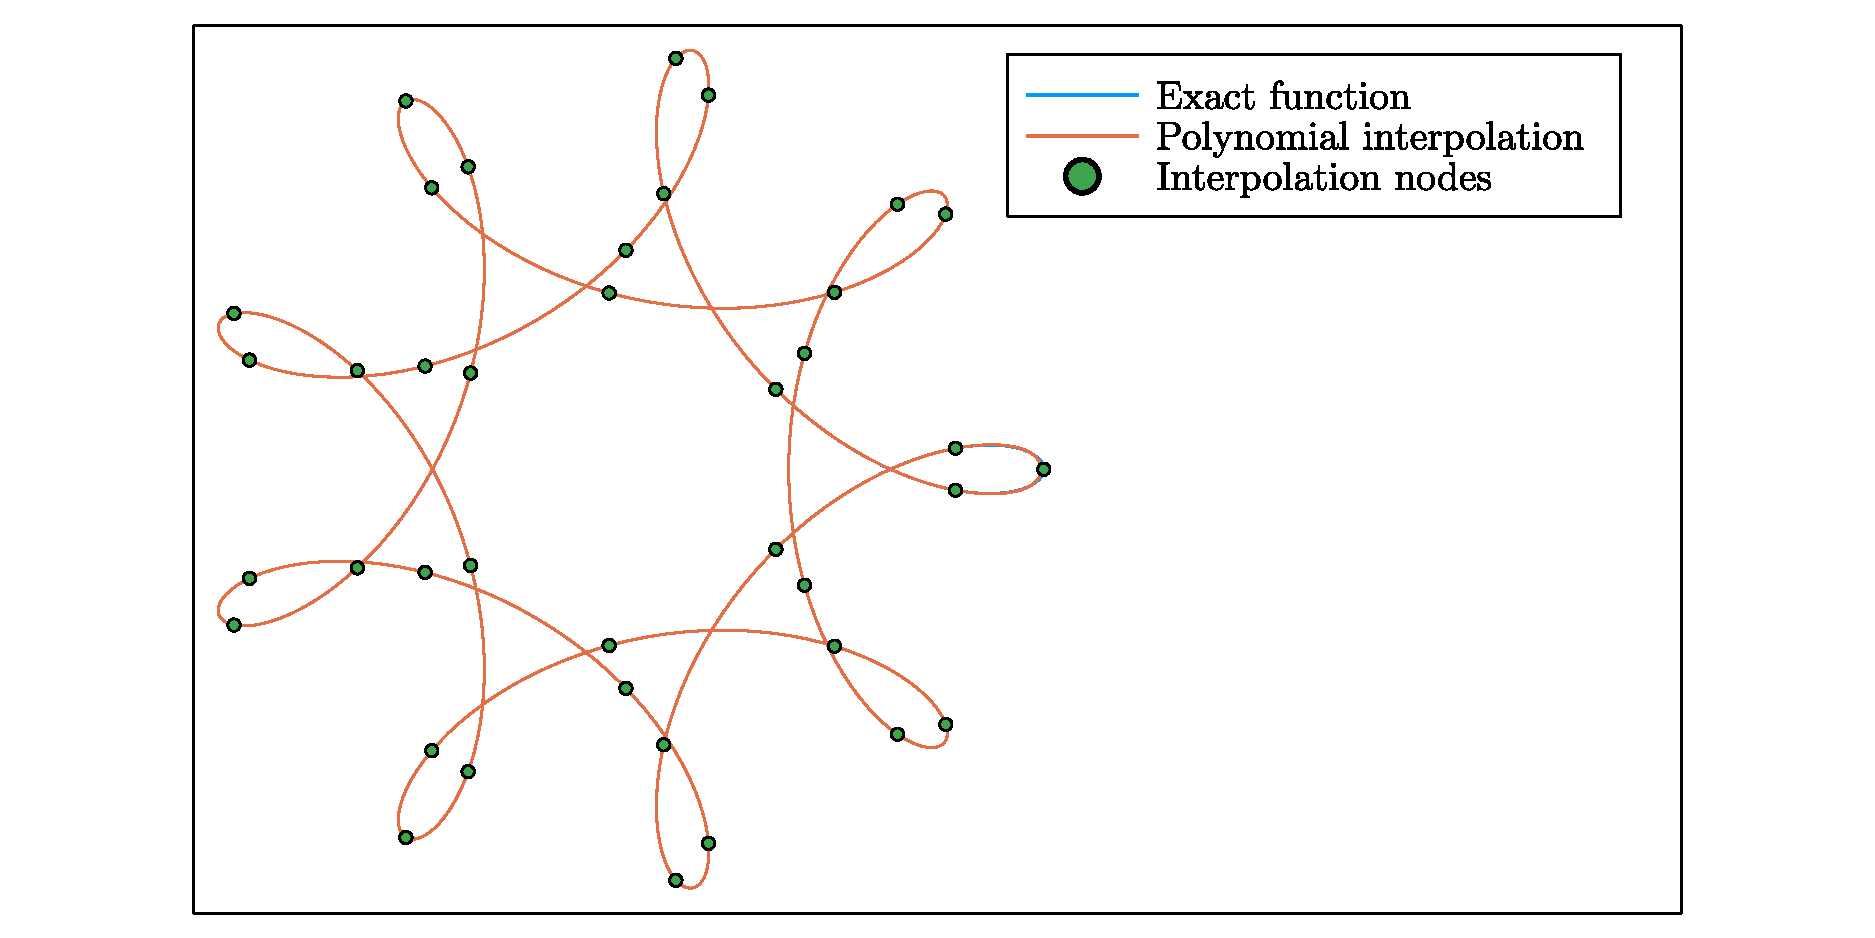
\includegraphics[width=0.99\linewidth]{figures/interpolation.pdf}
        \caption{Solution for \cref{exercise:parametric_interpolation}.}%
        \label{fig:parametric_interpolation}
    \end{figure}
\end{compexercise}

\begin{compexercise}
    [Modeling the vapor pressure of mercury]
    \label{exercise:approx}
    The dataset loaded through the following Julia commands contains data on the vapor pressure of mercury as a function of the temperature.
    \begin{minted}{julia}
    import RDatatets
    data = RDatasets.dataset("datasets", "pressure")
    \end{minted}
    Find a low-dimensional mathematical model of the form
    \begin{equation}
        p(T) = \exp \bigl( \alpha_0 + \alpha_1 T + \alpha_2 T^2 + \alpha_3 T^3 \bigr)
    \end{equation}
    for the pressure as a function of the temperature.
    Plot the approximation together with the data.
    An example solution is given in~\cref{fig:pressure}.
    \begin{figure}[ht]
        \centering
        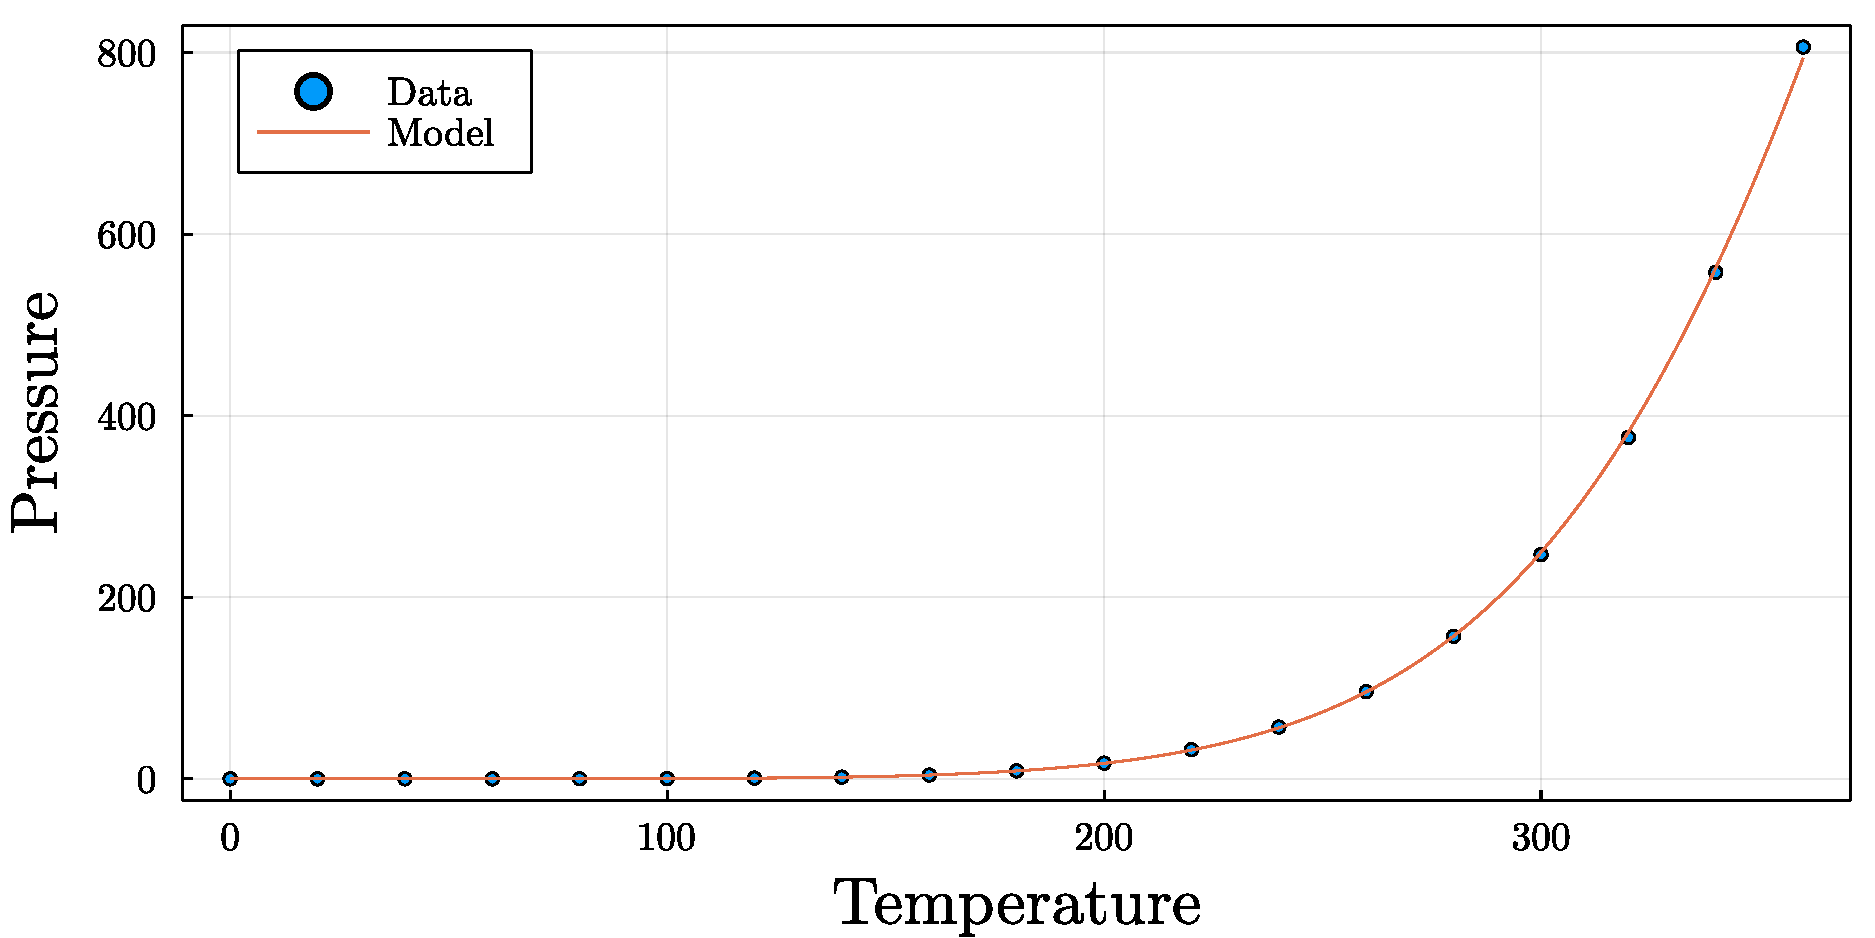
\includegraphics[width=0.75\linewidth]{figures/pressure_model.pdf}
        \caption{Solution for \cref{exercise:approx}.}%
        \label{fig:pressure}
    \end{figure}
\end{compexercise}

\section{Discussion and bibliography}
A comprehensive study of approximation theory would require to cover the $L^{\infty}$ setting
as well as other functional settings.
A pillar of $L^{\infty}$ approximation theorem is Chebyshev's equioscillation theorem, which we alluded to in~\cref{remark:cheb}.
An excellent introductory reference on approximation theory is~\cite{magnus} (in French).
See also~\cite[Chapter 10]{MR2265914} and the references therein.
